%%%%%%%%%%%%%%%%
% Ph.D. thesis %
%%%%%%%%%%%%%%%%

%\documentclass[11pt,openright,twoside,letterpaper,onecolumn]{report} %% USE THIS FOR DOUBLE SIDED
\documentclass[11pt,openright,oneside,letterpaper,onecolumn]{report}  %% USE THIS FOR SINGLE SIDED

\newcommand{\thesistitle}{Essays on Comparative Politics Methodology}
\newcommand{\thesisauthor}{Eduardo L. Leoni}
\newcommand{\thesisyear}{2009}

%%%
%%% Packages
%%%
%\usepackage[dvips]{epsfig}
\usepackage{amsmath}
\usepackage{named}
\usepackage{fancyhdr}
\usepackage{afterpage}
%
% We use the hyperref package and customize it for optimal PDF 
%
%%\usepackage[dvipdfm,pdftitle={\thesistitle},pdfauthor={\thesisauthor},pdfpagemode={UseOutlines},letterpaper,bookmarks,bookmarksopen=true,pdfstartview={FitH},bookmarksnumbered=true,]{hyperref}
\usepackage[pdftitle={\thesistitle},pdfauthor={\thesisauthor},pdfpagemode={UseOutlines},letterpaper,bookmarks,bookmarksopen=true,pdfstartview={FitH},bookmarksnumbered=true,]{hyperref}

%%%
%%% Margins
%%%
\paperwidth=8.5in
\paperheight=11in

% 1in + hoffset + oddsidemargin + textwidth + marginparsep + marginparwidth
% For PhD at Columbia we have single side theses and 1.5in left margin
% The settings below leave 1.5 inch margin at the left and 1 inch at the right 
% for US Letter paper
\setlength{\hoffset}{0.0in}
\setlength{\oddsidemargin}{.5in}
\setlength{\textwidth}{6in}
\setlength{\evensidemargin}{0mm}

% 1in + voffset + topmargin + headheight + headsep + textheight + footskip 
% For PhD thesis we also need an extra inch at the bottom
% 1inch = 72 pt
\setlength{\voffset}{0.0in}
\setlength{\topmargin}{.0in}
\setlength{\headheight}{14pt}
\setlength{\headsep}{22pt}
\setlength{\textheight}{8.5in}
\setlength{\footskip}{0pt}

%%%
%%% Spacing
%%%
%%\newcommand{\singlespace}{\renewcommand{\baselinestretch}{1.15} \small \normalsize}
\newcommand{\oneandhalfspace}{\renewcommand{\baselinestretch}{1.3} \small \normalsize}
% \newcommand{\doublespace}{\renewcommand{\baselinestretch}{1.5} \small \normalsize}
\newcommand{\normalspace}{\doublespace}
\footnotesep=1\baselineskip

%%%
%%% Counters depth
%%%
\setcounter{secnumdepth}{3}
\setcounter{tocdepth}{3}

%%%
%%% Title page.
%%%
\newcommand{\thesistitlepage}{
    \normalspace
    \thispagestyle{empty}
    \begin{center}
        \textbf{\LARGE \thesistitle} \\[1cm]
        \textbf{\LARGE \thesisauthor} \\[8cm]
        Submitted in partial fulfillment of the \\
        requirements for the degree \\
        of Doctor of Philosophy \\
        in the Graduate School of Arts and Sciences \\[4cm]
        \textbf{\Large COLUMBIA UNIVERSITY} \\[5mm]
        \thesisyear
    \end{center}
    \clearpage
}

%%%
%%% Copyright page.
%%%
\newcommand{\thesiscopyrightpage}{
    \thispagestyle{empty}
    \strut \vfill
    \begin{center}
      \copyright \thesisyear \\
      \thesisauthor \\
      All Rights Reserved
    \end{center}
    \cleardoublepage
}

%%%
%%% Abstract page.
%%%
\newcommand{\thesisabstract}{
    \thispagestyle{empty}
    \begin{center}
    \textbf{\LARGE ABSTRACT} \\[1cm]
     \textbf{\LARGE \thesistitle} \\[1cm]
     \textbf{\LARGE \thesisauthor} \\[1cm]
    \end{center}
    The abstract goes here.
The abstract goes here.
The abstract goes here.
The abstract goes here.
The abstract goes here.
The abstract goes here.
The abstract goes here.
The abstract goes here.
The abstract goes here.
The abstract goes here.
The abstract goes here.
The abstract goes here.

    \cleardoublepage
}

%%%
%%% Miscellaneous
%%%
\newcommand{\draft}{
    \renewcommand{\normalspace}{\singlespace}
    \normalspace
    \chapter*{Draft. Version \today}
\clearpage }



%%% Eduardo's modifications
\usepackage{graphicx}
\usepackage{natbib}
\usepackage{epigraph}
\setlength{\epigraphwidth}{.7\textwidth} 
\newcommand{\epi}[2] {
  \singlespace
  \epigraph{#1}{#2}
  \doublespace
}
\usepackage{setspace, fullpage}
%% single space is defined in setspace, redefining it here
\renewcommand{\singlespace}{\renewcommand{\baselinestretch}{1.15} \small \normalsize}
\renewcommand{\doublespace}{\renewcommand{\baselinestretch}{1.5} \small \normalsize}
%landscape package
\usepackage{pdflscape}
\usepackage{subfigure}
\newcommand{\comment}[1]{ {\textcolor{red}{\huge $\Rightarrow$}} {\textcolor{red}{{\scriptsize #1}}}}
\usepackage{amsmath}
\usepackage{latexsym}
\newenvironment{eqn1}{
  \singlespace
  \begin{eqnarray*}{}}{\end{eqnarray*}
  \normalspace
}


\begin{document}

% For the first pages we do not have numbering 
\pagestyle{empty}

\thesistitlepage
\thesiscopyrightpage

\thesisabstract

% In the "roman-numbered" section of the thesis, we have numbers at the bottom
% and we have to reduce the textheight of the text to make space for the number

\pagenumbering{roman}
\pagestyle{plain}

\setlength{\footskip}{0.5in}

\setcounter{tocdepth}{2}
\renewcommand{\contentsname}{Table of Contents}
\tableofcontents
\cleardoublepage

\listoffigures
\cleardoublepage

\listoftables 
\cleardoublepage

%%%
%%% Acknowledgments
%%%
~\\[1in] % hack to put space at top.
\textbf{\Huge Acknowledgments}\\

\noindent 
The acknowledgments go here.
The acknowledgments go here.
The acknowledgments go here.
The acknowledgments go here.
The acknowledgments go here.

\cleardoublepage

%%%
%%% Dedication page
%%%
\thispagestyle{plain}
\strut \vfill
\centerline{\LARGE 
Dedication text
}
\vfill \strut
\cleardoublepage

%\draft   % Generates a draft version in single-space

%%%
%%% BODY
%%%
\pagestyle{headings}
\pagenumbering{arabic}

%
% In the "arabic" section of the thesis, we do not have numbers at  the
% bottom and we want to use the full length of the page to avoid vbox
% underfulls. We use the fancyheaders package to adapt the headers
% according to the  Columbia requirements.
%
\setlength{\textheight}{8.5in}
\setlength{\footskip}{0in}

% We change the pagestyle 
\fancypagestyle{plain} {%
\fancyhf{}
\fancyhead[LE,RO]{\thepage}
\fancyhead[RE,LO]{\itshape \leftmark}
\renewcommand{\headrulewidth}{0pt}
}
\pagestyle{plain}

\chapter{Introduction}
\label{section:intro}
The introduction goes here.
The introduction goes here.
The introduction goes here.
The introduction goes here.
The introduction goes here.
The introduction goes here.
The introduction goes here.
The introduction goes here.
The introduction goes here.
The introduction goes here.
The introduction goes here.
The introduction goes here.
The introduction goes here.
The introduction goes here.
The introduction goes here.
The introduction goes here.


\part{The Statistical Analysis of Electoral Coalitions}
\label{sec:corpus}

% \title{The Statistical Analysis of Electoral Alliances}



% \author{Eduardo L. Leoni \\Department of Political Science\\
% Columbia University   \\
% 7th Floor, International Affairs Bldg. \\
% 420 W. 118th Street \\
% New York, NY 10027 \\
% %% Mail Code 3320 \\
% email: ell2002@columbia.edu}
% \date{}

% \maketitle \thispagestyle{empty}
% \bigskip
% \bigskip

% \abstract{In this paper we derive a statistical model from  an expected utility theory of electoral coalition formation in proportional representation systems. The theory predicts that parties are more likely to form a coalition if they are ideologically closer to each other. In addition, there is a party specific threshold that tells us how far the other party can be located and still asked to form a coalition. This threshold depends on the share of votes the party is expected to get and the magnitude of the district.  The statistical model we derive  is able to simultaneously estimate the ideological position of parties and the structural parameters relating  district magnitude and party size to coalition formation. We apply the model to the Brazilian local legislative elections of 2000 and find broad support for our hypotheses. Ideological distance, district magnitude and party vote-shares have negative effects on the likelihood of coalition formation. Moreover, the mean party locations derived from the model are highly correlated with the party locations estimated using roll call data in the national legislature. We also present arguably the first estimates of state-level positions of Brazilian political parties, and find that they are broadly consistent with hypotheses gathered from the Brazilian politics literature.}

% \end{titlepage}


%%TO DO
%% How is the number of seats decided?



%%Graham p.148 First, citizens divided politically not because of party loyalties, much less ideological considerations, but because of personal ties, making party labels seriously misleading at both the local and the national level. Second, power flowed simultaneously ``downwards'' from the Cabinet through the provincial president and ``upward'' from local bigwigs to the president and Cabinet in eddies and swirls that defy simple summary.

%\doublespace
%POOLE
%(1) a deterministic component that is a function of the distance between the 
%legislator and a roll call outcome; and (2) a stochastic component that represents the 
%idiosyncratic component of utility.
%Jackman on gelman's blog http://www.stat.columbia.edu/~cook/movabletype/archives/2004/11/ideal-point-mod.html
% One of the things I like about the setup in my work with Doug & Josh is that (1) our statistical model falls out of a fairly standard formal-theoretic approach to roll call voting (the Euclidean spatial voting model with quadratic utilities over outcomes and local/conditional independence); (2) our setup maps directly onto the 2 parameter IRT model from educational testing, about which much is known... In this sense our approach is a little more model-driven than data-driven (i.e., contrast naive MDS or factor analysis or clustering etc). My experience is that anything too data-driven in this field tends to run into trouble within political science because it while it is one thing to toss more elaborate statistical setups at the roll call data, they tend to lack the clear theoretical underpinnings of the Euclidean spatial voting model. Put differently, what is the model of legislative decision-making that underpins any given statistical model?

% What behavioral/political assumptions or processes suggest that we ought to do this when we model the data? The point here is that things that sometimes make good sense or seem attractive from a statistical perspective will often into a wall of skepticism from Congress people who like to see things built up from ground zero (legislators' utility functions...). 

%Gelman : I agree with you completely on the desirability of an individual-level "agent" model, which ideally (as in your work) can imply a statistical model.

% \begin{quote}
%   A coalitional structure is a partitioning of the set of players into a collection of groups, 􏰂 = (G j ) m j =1 , such that everybody is in some group ( ∪ m j =1 G j = N ) and no one is in two groups (G j ∩ Gk = ∅ for j ̸= k). Typically, we assume that a parti- tioning is defined uniquely up to the reordering of cells and of individuals within cells (thus {{1,2},{3,4}} is considered the same partition as {{4,3},{1,2}}). Let the set of all such parti- tions be given by G . For a population of size n, the cardinality of G is then given by the Bell number (Rota 1964), a number that grows very rapidly in n. The set of partitions for n = 4 is 15. For a 100-person senate, the Bell number is on the order of 10116 (Weisstein 2005).
% \end{quote} \citep{humphreys:2008}

% \begin{itemize}
% \item Parties decide, not ``coalitions''
% \item Spatial distance + valence matter
% \item Simplify the partition problem into binary decisions
% \item Formalize what assumptions are being made
% \end{itemize}

% For concreteness, let's assume there are three parties in the polity. We are interested on the parties' decisions to form electoral coalitions. 

% The possible partitions with three parties are:

% \begin{verbatim}
% {a,a,a} (A coalition of all parties)
% {a,b,a} (Parties 1 and 3 join a coalition a. Party 2 competes alone.)
% {a,a,b}
% {b,a,a}
% {a,b,c} (Each party competing separately)
% \end{verbatim}

% We are interested in casting the decision of which coalition structure to form in terms of each of the individual parties' decision to join a specific coalition. Note, in addition, that one can observe only one of those coalitional structures at each coalition opportunity for the parties. The number of possible coalitional structures, or set partitions, possible  is given by the Bell number $B(n)$\citep{rota:1964}. This number will grow very fast. With four parties, the number of possible partitions is 15; with seven (the number of effective parties in Brazil) it is 877. With 10 parties (half the number of parties represented in the Brazilian lower chamber) the Bell number is  115975. Without further simplifications it is  extremely difficult analyze all coalition decisions when the number of parties is moderate to large as in the Brazilian case.

% Therefore, we should look into ways to simplify the individual parties decisions. First, given that a particular coalition forms, what must be true about the utilities of the parties involved? This depends on the utility functions of the parties and on the particular game being played by the parties when forming coalitions.

% I illustrate the bias in traditional methods and apply a permutation test to one practical 
% example. Scholars in recent years have used group vs. subgroup comparisons to explore the 
% impact of federal forms of government on legislative party systems. The basic arguments are 
% as follows. Federal forms of government create and/or strengthen state-level (or province- 
% level) interests. Legislators in many national Congresses are accountable to state-level actors 
% for nomination, election, or career advancement. Consequently, national parties may split 
% on questions that mobilize pressure or that greatly affect state interests. To the extent that 
% these forces are at work, national-party cohesion should be lower because of the federal 
% form of government. 
% One country where this argument has been applied is Brazil. A federal republic with 
% 26 states and a federal district, Brazilian state politics have been characterized as having 
% important national effects. Brazilian federalism places key political resources in the hands of 
% state actors, granting them influence over the behavior of national legislators and weakening 
% national-party leaders (Mainwaring 1997, 1999; Selcher 1998; Souza 1998; Ames 2001; 
% Samuels 2002). For example, initial nominations to run for Congress and access to free 
% media time for campaign advertisements are both controlled by state parties. Similarly, state 
% governors distribute many political jobs, including coveted directorships of state agencies. 
% Consequently, “Politicians of the catchall parties focus a lot on state and local issues, so they 
% are less likely to toe the line of the national party leadership” (Mainwaring 1997, p. 83). As 
% a result, “. . .[f]ederalism influences the party system because most key decisions are made 
% at the state level and abundant resources are allocated at this level” (Mainwaring 1999, 
% p. 263). 


% These numbers, large as they seem, pale when confronted to what could have happened. There are more than two billion possible coalitions with two or more parties that can form in a party system with 31 parties. The number of possible ways to arrange these parties into electoral coalitions is orders of magnitude larger.\footnote{The number of possible partitions of a set of size $N$ is the Bell number of $N$\citep{rota:1964}.} Even if we concentrate on the 8 largest parties in Brazil, there are more than four thousand different coalitional structures that can emerge in each of the 5559 local elections in 2000. In this paper, we argue that a well grounded theoretical model can help simplify the statistical analysis while aiding in the interpretation of the results. %The main output of our model are estimates of the ideological positions of parties in each of the 26 Brazilian states.

% \begin{quote}
% In contrast, the spatial theory of voting is a \emph{theory of behavior}  that states that \emph{if} a set of assumptions holds, \emph{then}  voters should behave ina certain way \emph{and} we should observe certain types of outcomes. It is a theory that makes predictions that can be tested.\citep[p.9]{poole:2005}
% \end{quote} 

% \begin{quote}
%   Brazil has long been the case of most robust federalism in Latin America \dots By robust federalism, I mean that, during democratic periods, mayors and governors have been powerful actors with significant autonomy vis-à-vis the federal government and with significant resources. The catchall parties are decentralized, and parties and politicians generally follow a logic of federalism. Many of their actions are determined more by what goes on in their own states than by what goes on in national politics. In fact, the national parties are still to a considerable extent a federation of state parties.\citep[p.83]{mainwaring:1997a}\end{quote} 


% * Why do parties form coalition in advance of elections?
% * Coalition formation as surplus of votes sharing.

%\singlespace
\epi{Brazil is very uneven,  just a mess. One cannot understand it.}{Federal deputy and mayor Luciano Castro (PR-RR), commenting on the different political alliances at the national and local levels in Brazil. \\ Folha de São Paulo, June 29th \citeyear{bragon:2008}.}

\epi{(C)itizens (are) divided politically not because of party loyalties, much less ideological considerations, but because of personal ties, making party labels seriously misleading at both the local and the national level. }{\citet[p.148]{graham:1990} on political parties in 19th century Brazil.}
%\doublespace


Why do parties form coalitions?  Research into this question in comparative politics has mainly focused on the formation of \emph{government} coalitions in  parliamentary systems \citep{martin:2001a} and coalition support for the president in separation-of-powers systems  \citep{neto:2006,altman:2000}.  More recently, some attention has been paid to the electoral coalition agreements among parties in parliamentary systems \citep{blais:2008,golder:2006a}. 

In this paper, we focus on the electoral alliance decisions in local legislative elections in Brazil. Building on pioneering work by \cite{soares:1964}, the alliance formation theory we propose has the following characteristics. We assume that parties  have ideal points in a one-dimensional policy space. When forming alliances, parties want to maximize the number of seats won in the election while minimizing the ideological distance between the alliance members' ideal points. The incentives for alliance formation depend, then, on the ideological preferences of the potential alliance partners and the constraints imposed by political  (the expected party share of the votes) and institutional (the magnitude of the district) context. We derive a statistical model from these assumptions, which allows us to estimate both the spatial location of parties and the structural parameters of the model.

The statistical model we propose is closely related to ideal point estimation methods that rely on roll call data. Such models require  repeated decisions by the same actors in a large number of elections. The massive data available from the Brazilian local legislative elections provide us an excellent opportunity to estimate models of electoral alliance formation. In the elections of 2000, 368 thousand  candidates competed  for the  60 thousand  municipal legislators seats available in the more than five thousand independent elections (one per municipality) across the nation. The number of seats in each election varied from 9 (the constitutionally mandated minimum) to 55.  The number of candidates in each election ranged from 9 (in São Julião, Piauí state) to 1095 (in São Paulo, São Paulo state).  Candidates competed as members of 31 political parties under open-list proportional representation using the D'Hondt method. Parties were free to form  pre-electoral alliances (\emph{coligações}) in each election. There were 2845 different electoral alliances formed in the 2000 elections.

Since local political institutions in Brazil follow a separation-of-powers structure, we argue that these alliances do not form in order to attain a majority in the legislature. These pacts, after all,  are frequently different from those agreed upon for the competition for the Mayoral offices that occur simultaneously with the local legislative elections.  We argue instead that electoral alliances are simply pre-electoral agreements to share surplus votes when translating votes to seats. 

We find that there is an important ideological component to the parties' decisions to form pre-electoral alliances. Alliances more frequently arise between parties that are closer to each other in the ideological space. The overall party ordering estimated using the alliance data is highly correlated with the positions estimated using roll calls in the national legislature, giving some face validity to the model.  We also find that the institutional and political contexts, specifically the district magnitude and the size of the political party in the district, are just as important to the alliance decisions. 

The paper is structured as follows. First we outline the institutional features of local legislative elections in Brazil and briefly summarize the literature on this question. We then discuss the problems  of measuring ideology in Brazil and argue that the alliance data is a potentially good source for estimating party ideal points. Next, we present our statistical model of alliance formation and show the results from estimating our model using the 2000 elections. We  conclude by discussing possible  extensions to our model and its applicability in other contexts.

\section{Electoral alliances in Brazil}
\label{sec:measuring-ideology}


In the 2008 election for mayor in the Brazilian fourth largest city, Belo Horizonte, the two main opposing parties in Brazil -- PT (Workers Party) and PSDB (Social Democratic Party) -- formed an (informal) alliance.  If one looks at roll calls in Congress, these parties couldn't be farther apart \citep{leoni:2002}. Yet, an alliance between the state governor (Aécio Neves, PSDB) and the then mayor\footnote{Executive political positions in Brazil (mayors, governors and Presidents) can only be re-elected once.} (Fernando Pimentel, PT) was formed to (successfully) elect Márcio Lacerda (PSB) as mayor. 

The dissonance between local and national politics is seemingly maddening even for professional politicians and academics. In this paper, however, we show that there is an ideological structure in the electoral alliance decisions in local legislative elections in Brazil.  The theory we propose is simple, taking into account electoral imperatives and ideological preferences. In addition, since these decisions are made by the rank-and-file of the political parties, this analysis of alliance decisions serves to illuminate the interplay of politics at the national and regional levels. 

Local legislators in Brazil are elected under open-list proportional representation using a modified D'Hondt system. In this system,  voters  cast their vote for a specific candidate or for a political party. Votes are then aggregated up to the electoral list. The D'Hondt formula is used to distribute seats to lists, while  candidates within each list are ordered according to how many individual votes they received in the election.  The only modification to the D'Hondt system is that parties/alliances that received less than one ``electoral quotient'' (sum of valid votes divided by the number of seats) do not receive any seats. This means that there is an effective threshold of 1/number of seats, ranging from 11 \% in the smallest cities to 2\% in the largest city. This provides a substantive incentive for small parties to form alliances in small cities. 

The mechanical effect of the modified D'Hondt system on total party shares of local legislators in Brazil is plotted n Figure \ref{fig:comp}.  Only the three largest parties in Brazil (PSDB, PMDB and PFL) are net winners of seats if seat assignments where calculated without electoral alliances.   

 \begin{figure}
  \centering
  \includegraphics[width=.5\textwidth]{/Users/eduardo/reps/Brazilian-Local-Elections/results/Vereador/2000/comparisonPoints.pdf}
  \caption{The percent of votes for parties in Brazil in the 2000 elections summed over all municipalities plotted against .  }
  \label{fig:comp}
\end{figure}


% There are N votes in an election to select M legislators. 
Invalid votes and abstentions are excluded from the calculations. Votes are cast for individual candidates or parties, but  87\% of the voters select a specific candidate. All votes are aggregated up to electoral lists. Electoral lists may be made up by more than one party, joined together in an electoral alliance (\emph{coligação}). Fundamentally, an electoral alliance is an agreement to share ``surplus'' votes across political parties. Perhaps as importantly in the largest municipalities, parties also agree to share the assigned free television time they have. Elections for mayors and local legislators are held concurrently in the midterm of the national elections.

That parties and alliances play a minor role in elections in Brazil can be glanced from political advertisement in Brazil.  Figure \ref{fig:add_sp} shows a typical political advertisement that can be found in the Brazilian streets during election season. The add is dominated by the face,   name and number of the candidate. The number is important, since knowing it is necessary for the voter to cast his/her vote to a specific candidate in the voting booth. Brazil uses electronic voting since the 1996 elections. The party of the candidate occupies a very small space in the add. Finally, there is usually some reference to the candidate of the Executive post (Mayor, in this case). 

\begin{figure}
  \centering
  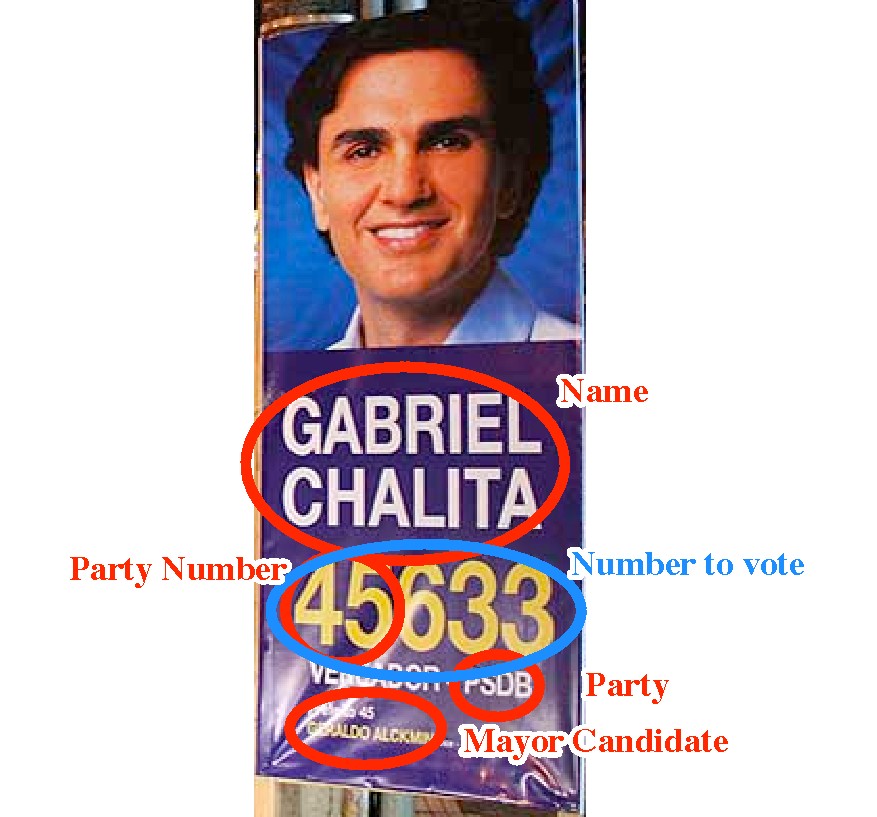
\includegraphics[width=.5\textwidth]{../images/alliances/propaganda_sp.pdf}
  \caption{Add for a Vereador candidate in São Paulo. Note that the picture of the candidate covers most of the add and the party label is comparably very small. The alliance is nowhere to be seen.}
  \label{fig:add_sp}
\end{figure}


There is a growing literature on the analysis of electoral alliances in Brazil. The pioneering work was done by  \citet{soares:1964}. Making use of the \citet{downs:1957}'s spatial theory of democracy, Soares proposed two theories/hypotheses to account for electoral alliance formation in Brazil.  The  ``cost minimization theory'' hypothesis  states that parties will form alliances 
in order to maximize their seat shares given the number of votes they expect to get in the forthcoming elections. The ``ideological resistance'' hypothesis states that parties prefer to form alliances with parties that have similar ideological positions. 

That article ignited a cottage industry of papers studying electoral alliances in Brazil, which has been particularly active in the recent period.\footnote{\citet{miguel:2007} provide an excellent review of the literature.} This literature, however, faces a couple of serious short-comings. First, the ideology measures used are hard to replicate and not explicitly linked to any sort of political behavior. Secondly, the theoretical development seem to have stagnated with Soares article from four decades ago. ``Ideological resistance'' and ``cost minimization'' are seen as ``either-or'' propositions, without an integrated way to think about how they both might affect party behavior. A final problem is the lack of a statistical model, without which the  importance of ideology and/or  ``cost minimization'' hypotheses on party behavior cannot be ascertained. 






\section{On   ideology and its measurement}

Ideology in modern political science is currently thought as a theory of political behavior. We  start by assuming that the policy space is high dimensional. For instance, views about international trade, government support for child care, abortion, taxes, etc, can all vary independently across voters and politicians. However, research  has shown that most of the issues governing the day are highly correlated, so that when one analyzes the actions of decision makers, just one or two dimensions might be sufficient to explain most of the behavior. This low dimensional space is called ``predictive'', ``basic'' \citep[p.13-14]{poole:2005} or, most commonly, ``ideological'' space \citep{hinich:1994}.   

If we define ideological space as the predictive dimensions of political behavior, it is not surprising to note that state of the art measurement models of ideology derive ideal point estimates from observed political action. There is a long and noble tradition of measuring  ideology of legislators using their roll call votes.\citep[e.g.]{poole:1997}. \citet[p.355]{clinton:2004} go so far as stating that the ``primary use of roll call data is the estimation of ideal points.''  As these authors note, roll calls are effective measures for  describing  the behavior of legislators. There are a many other things that legislators do, of course. But roll calls are both readily available in many legislatures, and also important since they record preferences over actual policies. Researchers also use roll calls in order to \emph{test} spatial theories of political behavior.  In this tradition, one starts by formulating a (formal) theory of behavior, derives the implications of such theory and then estimates a model that follows from it.\cite[p.9]{poole:2005} 

One should note that there is nothing particularly special about roll call data: any other record of behavior that can be thought of as a consequence of the theory being tested is likely to be just as useful. What is in fact special about roll call data is the extraordinary quantity and time-span of such data  for the United States Congress and many other legislatures across the world.

% There is a well known problem with roll call data, however. If, for example, the agenda is controlled by the majority party leadership, bills that would divide the majority party are not likely to reach the floor. 

In Brazil a one dimensional model of roll call behavior seems  to fit well the data \citep{leoni:2002}.  The two-dimensional ideal points  for legislators in the legislative sessions from 1991 until 2006 are displayed in Figure \ref{fig:wnominate}, along with estimated cutting-lines\footnote{We used the \texttt{wnominate} \citeyear{poole:2007} \texttt{R} package to perform estimation and plots.} . The cutting-lines are estimates of the lines separating legislators voting \emph{Yea} from those voting \emph{Nay}.  A one dimensional model predicts correctly around 88\% of the roll call votes in the 1991-1996 session and 92\% in the legislative sessions from 1995 until 2006. 

\begin{figure}
  \centering
  \includegraphics[width=.9\textwidth]{/Users/eduardo/projects/BrazilianPolitics/trunk/dissertation/hip/wnominate_plot.pdf}
  \caption{\textsc{W-NOMINATE} ideal point estimates of the Brazilian Chamber of Deputies, 1991-2006. Note how, starting in the 1995-1998 session, cutting lines are almost all vertical and concentrated in a small portion of the state.}
  \label{fig:wnominate}
\end{figure}

The Figure is interesting for what it does \emph{not} show: from 1995 to 2002 the roll call cutting-lines almost never separate parties in the majority. The majority is located in the right side of the space in the 1991-2002 sessions and in the left side of the space in the 2003-2006 session.   Since roll calls do not split the majority parties, there is limited information available in them that is useful to differentiate parties \emph{within} the majority.

Another, more serious, problem is that the estimated ideal points can only be treated as such (ideological ideal points) if  roll call behavior is driven predominantly by spatial preferences. Let $i$ index legislators and $j$ index roll calls. A function linking preferences $x_i$ to roll call behavior $y_{ij}$ can be written as:

\begin{equation}
  \label{eq:3}
  y_{ij} = f(\alpha_j+x_i\beta_j +e_{ij})
\end{equation}

That is, the model assumes that only preferences drive behavior. More precisely, the errors $e_{ij}$ are independent and identically distributed. If, however, there is some sort of vote buying $z_{ij}$ that is not constant across legislators, then estimated ideal points will be biased. This would be of not much consequence if all we want is a description of roll call behavior, but insufficient if we want to test a theory of behavior. In the case of Brazil, part of the literature claims there is a \emph{quid pro quo} between Presidents and legislators.\citep{alston:2006,alston:2007,zucco:2007} Presidents  have the authority to withhold expenditures under the Brazilian Constitution, so, according to the argument in these articles, they have leverage when dealing with legislators.  Since such vote buying is in general inconsistent with pure spatial voting, the usual estimators of ideal points will lead to misleading estimates of preferences. This argument is more fully developed by \citet{zucco:2009}. He combines roll call data with a self-positioning of legislators measured using surveys and finds that the influence of ideology (as measured by the surveys) on roll call behavior of deputies has declined over time in Brazil. 

Another way to deal with the issue is to find data where such constraints (e.g. vote buying) are not as relevant. \citet{groseclose:2000}  argue that measuring ideology lop-sided roll calls in Congress are closer to the ``true'' preferences of legislators, and the difference between these preferences measured using lop-sided votes and preferences measured using non lop-sided serve as a measure of party influence on roll call behavior. More generally, we want to find behavior that is important  (behavior that ``matters'') but not overwhelmingly influenced by outside actors (e.g. the President).  In this vein,  \citet{monroe:2008} propose to measure ideal points using political text and speech; \citet{aleman:2009} use cosponsorship, that is, data on which legislators cosponsor each other bills, to estimate ideal points using singular value decomposition techniques; Finally \citet{saiegh:2009} uses survey data from political elites. 

Most of these measures, however, are restricted in their ability to estimate ideal points of small political parties. If there is only one or two legislators in Congress  that are members of a particular political party, for example, there is not sufficient information to estimate an ideal point for that party. For the same reason, it is usually impossible to estimate intra-party (e.g. cross-district) variation of ideal points using roll call data. There are simply not enough data. Zucco faces the same issues, relying on at most 250 legislators per legislature.  

The massive amount of data on party alliance behavior in local elections in Brazil, we argue, can  help us in this regard. In the next section we present a model of alliance formation. We   derive from it  a statistical model that is able to simultaneously estimate party ideal points and, as importantly, structural parameters that relate political context and structure to the likelihood of forming a alliance. Local alliance decisions are useful because  they reflect decisions by the rank-and-file of the party at  the lowest level of elected office in Brazil,  with arguably little interference from the nation-wide party leadership.

Figure \ref{fig:coalplot}  displays alliances decisions for the 31 parties competing in the 5559 local legislative elections in 2000 in Brazil. In the diagonal are the number of elections each party participated in. Each row displays the count of elections where the row-party formed a alliance with the column party. The parties are ordered  using a seriation algorithm that puts similar parties (in terms of alliance behavior) together.\footnote{We use the \texttt{seriation} function of the \texttt{cba} R package \cite{buchta:2006}.} The color scale displays the proportion of the alliances that includes the row-party that also include the column-party. For instance, more than 40\% of the alliances that the PCdoB formed also include the PT. On the other hand, only about 25\% of  the alliances formed by the PT also include the PCDOB.


The most important feature of the matrix is that it has relatively few zero entries. This  implies that ideology is far from being the overwhelming driver of alliance decisions. The main left wing party (PT)  formed alliances with the main right-wing party (PFL) in about 2\% of the elections it is a participant of. In fact, the PT (and only the PT)  formed at least one alliance with every other party in Brazil in the 2000 elections: from the trotskist  PCO  to the nationalist right wing PRONA. Nevertheless, it is immediately obvious that the parties have preferred partners. The communist parties PCB and PCdoB, for example, have the PT in their alliance in almost half the elections they participate in.  Alliance decisions, therefore, do seem to be  at least partly  driven by ideology. 
   
\begin{landscape}
\begin{figure}
  \centering
  \includegraphics[height=.9\textwidth]{/Users/eduardo/projects/BrazilianPolitics/trunk/dissertation/alliances/coalplot.pdf}
  \caption{Counts of alliance decisions in the Brazilian local legislative elections of 2000. Each cell  displays the counts of  alliances that include the row-party and the column-party. The color scale reflects counts as a  proportion of all alliances of the row party.}
  \label{fig:coalplot}
\end{figure}
\end{landscape}


\subsection{State level preferences}



Brazil is large federal country, with important regional variations in terms of economic and social structure. Thus, it is likely that there is also regional variation of party preferences across states. In the United States, for example, for a long time there was a noticeable split between southern and northern Democrats in the United States on civil rights issues\citep{poole:1997}. In the case of Brazil, many scholars argue that state-level actors are not only independent on local matters, but also have a great deal of influence on national level politics. \citet{mainwaring:1997a} calls this ``robust federalism'': 

\begin{quote}
  Brazil has long been the case of most robust federalism in Latin America \dots By robust federalism, I mean that, during democratic periods, mayors and governors have been powerful actors with significant autonomy vis-à-vis the federal government and with significant resources. The catchall parties are decentralized, and parties and politicians generally follow a logic of federalism. Many of their actions are determined more by what goes on in their own states than by what goes on in national politics. In fact, the national parties are still to a considerable extent a federation of state parties.\citep[p.83]{mainwaring:1997a}\end{quote} 


\begin{figure}
  \centering
  \includegraphics[width=1\textwidth]{/Users/eduardo/projects/BrazilianPolitics/trunk/dissertation/alliances/ufplotAll.pdf}
  \caption{Alliance dyads and roll calls in the national lower house by state.}
  \label{fig:coalplot}
\end{figure}

\citet{Samuels:2003} and \citet{abrucio:1998} argue that the legislative institutions at the national assembly, particularly the budgetary committees, are structured in order to privilege state-level actors. They argue that  elections for congress are based on state-wide districts and governors  are supposedly more influential on the election success of national legislators than the national parties or the President.   

Even if the governors themselves had little influence on roll call behavior, the extensive regional differences across Brazil are likely to have effects on the preferences of legislators, even for legislators from the same party. Using roll call data both from the Senate and from the Câmara, \citet{desposato:2003} found that national party cohesion is, in fact, lower than state-party cohesion. 

As show in the right panel of Figure \ref{fig:coalplot}, the alliance data set is much richer than the Câmara dos Deputados roll call data set for estimating district level preferences of the Brazilian parties. The parties and states in the figure are ordered by the number of alliances present in each party/state. Note that for none of the parties we have roll call information from every state. More worryingly, only about 6 or 7 parties have representatives from more than half the Brazilian states. The alliances data, on the other hand, covers every state  for the main political parties in Brazil. 



\section{A statistical model of electoral alliance formation}

In this  section we present a simple model of electoral alliance formation. There are $N$ individual parties competing in $M$ elections. Elections are held across $S$ states. We assume that parties first choose the largest set of parties that they are willing to form a alliance with. Parties that choose the same set $S_m$ form a alliance  $S'_m$. This can be  different from $S_m$, since it is not necessary that all parties in $S_m$  accept to join the alliance for a subset of the alliance to form.\footnote{We adopt the assumptions of the game named as  $\Delta$  by \citet{hart:1983}. Note, however, that in our model parties do not behave strategically. This assumption is similar to the independence of irrelevant alternatives in multinomial logit models. See \citet{train:2003} for a discussion.} Therefore, if  a alliance involving party $i$ and party $j$ is observed at election $m$, we know that $S_{im}=S_{jm}$ and $U_{im}(j\not\in S_{im})<U_{im}(j\in S_{im})$ and $U_{jm}(i\not\in S_{jm})<U_{jm}(i\in S_{jm})$ . Conversely, if parties $i$ and $j$ are not in the same alliance in  election $m$, we know that $S_{im} \neq S_{jm}$ and $U_{im}(j\not\in S_{im})>U_{im}(j\in S_{im})$  or $U_{jm}(i\not\in S_{jm})>U_{jm}(i\in S_{jm})$.   

We need a parametric form to proceed to empirical analysis. We define the utility for party $i$ of adding a party $j$ to the alliance as follows. We start by assuming that each party $i$ in state $s$ can be located at point $x_{is}$ in a one-dimensional policy space.  The utility function we propose has two additive components. The first is  the policy cost of forming a alliance with a party that has, in general, different policy positions from one's own. This cost is modeled as $-|x_{is}-x_{js}|$.  The second component is the non-spatial threshold parameter $v_{im}$ for party $i$ of adding party $j$ to the alliance in election $m$.  Party $i$ offers party $j$ a alliance proposal if:

\begin{eqnarray}
  \label{eq:u2}
  - |x_{is}-x_{js}| +  v_{im}&>&0
\end{eqnarray}

In more words, party $i$ will extend an offer to   party $j$  if and only if the  expected spatial cost is less than the threshold parameter $v_{im}$. This completes the deterministic component of the parties' utilities. To cast this decision in terms of a random utility model we add error terms $e^1_{ijm}$  and $e^0_{ijm}$   to  $U_{im}(j\in S_{im})$ and $U_{im}(j\not\in S_{im})$ respectively. These are the stochastic components of the utility functions. The probability that party $i$ extends an offer to party $j$ in election $m$ is then:

\begin{eqnarray}
  \label{eq:probit.i}
P(z_{ijm}) &=&P(-|x_{is}-x_{js}| +  v_{im} + e_{ijm}  >0)  \\
  &=&P(-|x_{is}-x_{js}|  +v_{im}   >-e_{ijm}  )
\end{eqnarray}

This is in general different from the probability that party $j$ extends an offer to party $i$:

\begin{equation}
  \label{eq:probit.j}
  P(z_{jim})=P(-|x_{is}-x_{js}| +  v_{jm}   >-e_{jim}  )
\end{equation}

Recall that we do not observe the offers being made, we only observe if parties $i$ and $j$ accept offers from each other. Let $y_{ijm}$ be a binary variable reflecting the observation that parties $i$ and $j$ formed a alliance in election $m$. Given our assumptions, we know this occurs only if the inequalities in equations \ref{eq:probit.i}  and \ref{eq:probit.j} are simultaneously satisfied. We further simplify the problem by assuming that $e_{ijm}$ and $e_{jim}$ are independent and have each variance 1 and mean 0. With this assumption we now have:

\begin{eqnarray}
  \label{eq:ru1}
  P(y_{ijm})=P(U_i(j \in S_{im})>U_i(j\not \in S_{im})) \cdot P(U_j(i\in S_{jm})>U_i(i\not\in S_{jm}))\\
  =P(v_{im}-|x_{is}-x_{js}|+e_{jim}>0) \cdot P(v_{jm}-|x_{is}-x_{js}|+e_{ijm}>0) \\
  =\Phi(v_{im}-|x_{is}-x_{js}|) \cdot \Phi(v_{jm}-|x_{is}-x_{js}|)
\end{eqnarray}

The threshold parameter is modeled as a function of party size. district magnitude and an election specific error term. We reason as follows. Let the (expected) proportion of votes for party $i$ in election $m$ be $p_{im}$. Let $z_{m}$ be the magnitude of the district in election $m$. Under the open-list  D'Hondt electoral system, candidates  from parties attaining less than $1/z_{m}$ votes do not get elected. Note that this happens even if  $p_{im}$ is greater than the proportion of votes necessary to elect the least successful candidate of some other party with a share of votes higher  than $1/z_{m}$.  Thus, the  D'Hondt system favors large parties/alliances at the expense of smaller parties. However, the degree of proportionality in proportional representation systems increases with district magnitude. Hence, the incentives for alliance formation decrease with $\frac{p_i}{1/z_{m}}=p_i\cdot z_{m}$, and this effect should get smaller as $p_i$ and/or $z_{m}$ get larger. We model this multiplicative effect using natural logs\footnote{We will exclude parties with zero votes from the estimation.}:

\begin{equation}
  \label{eq:1}
  v_{im}=\gamma_1 +\gamma_2\log(p_{im})+\gamma_3 \log(z_m)+g_m
\end{equation}

Parameter $\gamma_1$ is the overall intercept of the statistical model. We expect both $\gamma_2$ and $\gamma_3$ to be negative. The error term $g_m$ is assumed to have a normal distribution with variance $\sigma_{city}^2$. 

\section{Estimation}

We observe parties forming alliances in  $M$ separate elections, nested within the 26 Brazilian states. The decisions in each election are represented in a  $Y_m$ lower-triangular matrix.  The parameters $x$ and $\gamma$ are unobservable quantities and have to be estimated.  Since these quantities are not observed,  the estimation turns out to be a difficult maximization problem.  For each additional party $i$ in state $s$ we have to estimate  an additional parameter  $x_{is}$. And for each additional election $m$ we have a new $g_m$ to estimate.  Thus, as the sample size increases, so does the number of parameters in the model. This causes problems to the maximum likelihood estimation.\citep[p.358]{clinton:2004} These are, however, of not very much consequence to the Bayesian estimation, since the Bayesian approach holds the data fixed and approximations, when necessary, depend only on the number of simulations performed and not on the size of the data.  

The likelihood of the model is: 

\begin{eqnarray}
  \label{eq:llike}
  L(x,\gamma|Y)=\\
\prod^M_{m=1}\prod^N_{i=2}\prod^{i-1}_{j=1}  \{\Phi( v_{im}-|x_{is}-x_{js}|+g_{m})\Phi( v_{jm}-|x_{is}-x_{js}|+g_{m})\}^{y_{ijm}}\\
  \times\{(1-\Phi( v_{im}-|x_{is}-x_{js}|+g_{m})(1-\Phi( v_{jm}-|x_{is}-x_{js}|+g_{m})\}^{(1-y_{ijm})}
\end{eqnarray}

Estimating state-specific ideal points for the parties introduces  comparability problems, since  parties in any given state interact only with other parties in the same state. Thus, to compare party ideal point locations across states we need further assumptions. We follow \citet{martin:2002} in using a  hierarchical model. These authors use a  dynamic hierarchical prior  on  ideal points, more specifically  a random walk prior that is conditional on the ideal point in the last period.(p. 135) In our case, instead of time the relevant grouping structure is state. Since states are unordered,  the model is not dynamic (and therefore much simpler to estimate.) The prior for the  ideal point of party $i$ in state $s$ is:


\begin{equation}
  \label{eq:5}
  x_{is} \sim N(\bar x_{i},\sigma_x^2)
\end{equation}

Bayesian estimation requires us to specify prior distributions for all unknown parameters. We chose the following weakly informative priors \citep{gelman:2008} \footnote{Note that we follow the advice of \citet{gelman:2004} on the estimation of the variance parameters.} $\bar x_i \sim N(0,10^2)$; $\gamma_k\sim N(0,10^2)$;   $g_m\sim N(0,\sigma_{city}^2)$;  $\sigma_{city}~\sim~U(0,10)$;   $\sigma_x~\sim~U(0,10)$.

We still need to set restrictions on the policy space due to additive and multiplicative aliasing to identify the model.\citep{bafumi:2005}  In a one-dimensional policy space, two linear restrictions are required in order to identify such models.\citep{rivers:2004} We choose to fix the prior mean ideal points of two of the parties, Partido dos Trabalhadores (Workers Party, PT) and Partido da Frente Liberal (Liberal Front Party, PFL).  These  are  the most important parties at, respectively, the left and the right of the Brazilian political spectrum.\citep{figueiredo:1995}   The  scale is set so that  $\bar x_{pt}$   is  $-1$  $\bar x_{pfl}$ is  $1$. 


We estimate the model using the general-purpose \texttt{JAGS} \citep{plummer:2007} software for Bayesian posterior simulation.\footnote{JAGS is a compiler for code written using the BUGS language. The code we used is displayed on the appendix.}  The identification constraints on $x$ are imposed after the simulations are complete, as suggested by \citet{bafumi:2005}. Specifically, we  calculate for each posterior simulation:

\begin{eqnarray}
   \label{eq:2}
   \lambda&=&\frac{\bar x_{pfl}-\bar x_{pt}}{2}\\
   \bar x_{i}^*&=&(\bar x_{i}-\bar x_{pt})/\lambda-1\\
   x_{is}^*&=&(x_{is}-\bar x_{pt})/\lambda-1\\
   \gamma^*&=&\gamma/|\lambda|\\
   \sigma^*&=&\sigma/|\lambda|
 \end{eqnarray}


 \section{Data issues and  preliminary results}
 \label{sec:results}  

 In this section we report the still preliminary results of estimating our model and some data challenges we are currently facing.
 
 \subsection{Data issues}
 \label{sec:data-issues}

\begin{description}
\item[Expected number of votes] At this preliminary stage we use the actual number of votes the party received in the election. In the future we will model expected party votes using the electoral results from past elections. Since: a) less than 15\% of the voters vote for parties instead of candidates and; b) of those voting for candidates, only a small proportion know the party of the candidate they voted for, we conjecture that the results would  change very little if  the previous vote is used. 
\item[Non-competing parties] We only model decisions where both parties received more than zero votes in the election. Our model, then, is conditional on entry. We argue that the decision to enter the competition can be usefully analyzed separately from the decisions to form alliances. 
\item[Very small parties]  In order to decrease computing time, we limit the analysis to the ten parties that received the most votes in the local legislative elections of 2000. In decreasing order of size: PMDB, PFL, PSDB, PPB, PTB, PT, PDT, PL, PPS, PSB. There are 103594 alliance dyads across the 5345 Brazilian municipalities in this subset of the data. 
\end{description}

\subsection{Preliminary results}

In Figure \ref{fig:mu} we compare the national party prior mean distributions ($\bar x$) to the party means estimated using roll call votes from the national level Câmara dos Deputados in 1999 and 2000.    The correlation coefficient between the two sets of estimates is around $0.8$.\footnote{We exclude from the calculations the positions for PFL and PT, since they are constrained to be 1 and $-1$ respectively.} The horizontal lines displays the estimation uncertainty of the alliance model (95\% confidence interval\footnote{FIX}) while the vertical lines  display the uncertainty of the roll call model. The confidence intervals for the alliance model are noticeably larger than those of the model using roll call data.   


\begin{figure}
  \centering
  \includegraphics[width=.4\textwidth]{/Users/eduardo/projects/BrazilianPolitics/trunk/dissertation/alliances/coalExample.pdf}
  \caption{Comparison of party ideal points estimated using data from a random subset of Brazilian municipalities and party ideal points estimated using roll call data from the national lower house (1999-2002). There correlation between the two sets of points is $.8$.}
  \label{fig:mu}
\end{figure}


The coefficients for the structural parameters of our model, number of seats and party size, have negative signs as expected. We display them in panel (a) of  Figure \ref{fig:coefs}. Larger parties and parties in municipalities with a larger number of seats are on average less likely to form alliances.  Panel (b) displays the standard deviation of the group level parameters. Note that the state level residual variation of party positions ($\sigma_x$) and municipality specific intercepts ($\sigma_{city}$)  are of roughly the same magnitude.   


\begin{figure}
  %%\centering
    \subfigure[Coefficients of the structural parameters.]{
      \includegraphics[height=.37\textwidth]{/Users/eduardo/projects/BrazilianPolitics/trunk/dissertation/alliances/bCIplot.pdf}
    }
    \subfigure[Standard deviation of the random effects.]{
      \includegraphics[height=.37\textwidth]{/Users/eduardo/projects/BrazilianPolitics/trunk/dissertation/alliances/sigma.pdf}
    }
  \caption{Bayesian confidence intervals for the parameters of the model. The dots mark the median of the posterior distributions. In panel (a) we display the structural parameters of the model. As expected, larger parties and parties in municipalities with large legislatures are on average less likely to form alliances. In panel (b), note that the random effects standard deviations are roughly of the same magnitude.  }
  \label{fig:coefs}
  \end{figure}  


To aid interpretation, we plot predictions from our model in Figure \ref{fig:strucpred}. Each panel displays the predicted probabilities for different combinations of party size. When both parties are small (top-left panel), each with 5\% of the votes, the probability of a alliance being formed is quite high. For example, there is a 50\% chance that parties of that size  will form a alliance if they are very close to each other and the number of seats available is at the minimum (9). However, this probability drops to around 10\% if there are 20 seats available. We can also see that the predicted drop in the probability of alliance formation as spatial distance increases  abrupt, highlighting the importance of spatial locations in the alliance decisions of parties in Brazil.

\begin{figure}
  \centering
  \includegraphics[width=.5\textwidth]{/Users/eduardo/projects/BrazilianPolitics/trunk/dissertation/alliances/predictions.pdf} 
  \caption{Predicted probabilities with 95\% Bayesian confidence intervals of alliance formation. The panels display the probabilities for different party sizes.  }
  \label{fig:strucpred}
\end{figure}

Since we are  the first to estimate state-level preferences of political parties in Brazil,  there are no other measures to compare ours to. Instead, we gather from the Brazilian politics literature and local news a set of  stylized facts/hypotheses about regional party preferences in Brazil that we should be able to find using the alliance data:

\begin{enumerate}
\item \label{f:ba} \textbf{PSDB in Bahia should be far from the PFL}. The main leader of PSDB in Bahia, Jutahy Magalhães Junior, is a long time foe of the head  of the  PFL in the state, Antonio Carlos Magalhães (no relation.) The dissension is so extreme that the PSDB in Bahia supported the PT candidate in the 1994 presidential race \emph{against} the PSDB candidate, Fernando Henrique Cardoso, who was ultimately elected along with Marco Marciel, a PFL politician,  as vice-president. 

\item \label{f:pe} \textbf{PMDB in Pernambuco should be on the right.} The main leader of the PMDB in Pernambuco, Jarbas Vasconcelos, is known to be on the right wing of the eternally fractured PMDB. The current Senate president and big-wig of the party, José Sarney, claimed in 2009\footnote{\url{http://blogdofavre.ig.com.br/2009/03/o-jarbas-hoje-e-mais-psdb-que-pmdb-diz-sarney/}, \url{http://www.chicobruno.com.br/index.php?data=2007-01-12}} ``Jarbas is closer to the PSDB than to the PMDB''. (The PSDB is usually placed to the right of PMDB in Braizl.)

%\item \textbf{PMDB in Paraná should be on the left.} The main leader of the PMDB in Paraná is Robero Requião, the current governor.

\item \label{f:mgrs} \textbf{Politics should be polarized in Rio Grande do Sul (RS) and consensual in Minas Gerais (MG).} \citet{renno:2004} studied two  municipalities in his PhD. dissertation, one in  Minas Gerais  and the other in Rio Grande do Sul. He found that in Caxias do Sul (RS)  politics was polarized  between ``the Workers’ Party and a alliance of the other parties''(p.25).  In Juiz de Fora (MG), on the other hand,   ``the political system \dots is organized around individual political leaders.  Politics is carried out mostly on a personalistic base and parties are weakly institutionalized.'' (p. 24) If these characteristics are more generally held in each state, we would expect politics to be more polarized in Rio Grande do Sul than in Minas Gerais. 
\end{enumerate}

In Figure \ref{fig:stateideology} we show the state-level estimated preferences of political parties in Brazil. The colored circles plot the positions of the four largest parties, while party labels plot the position of the remaining parties. The states are ordered by the range of party positions, which serves as a rough indicator of polarization of the state party system.  Consistent with hypothesis   \ref{f:mgrs}, we find that Rio Grande do Sul  is the second most polarized state while Minas Gerais is the second least polarized state. Confirming hypothesis \ref{f:pe}  the PMDB in Pernambuco is at the right of the local ideological space. Finally, in line with hypothesis \ref{f:ba},   the PSDB  is quite far from the PFL in Bahia.  

\begin{figure}
  \centering
  \includegraphics[width=1\textwidth]{/Users/eduardo/projects/BrazilianPolitics/trunk/dissertation/alliances/stateideology.pdf} 
  \caption{State party preferences. }
  \label{fig:stateideology}
\end{figure}


\section{Project outlook}
\label{sec:concl-proj-outl}

In this paper, we outlined a statistical model of electoral alliances and applied it to the case of Brazil. Using a Bayesian hierarchical model, we provided estimates of the structural parameters driving alliance behavior (party size and number of seats) and arguably the first state-level estimates of party ideological positions. Being the first unfortunately also means not having other measures to compare to. The results, however, are  consistent with hypotheses we gathered from the literature and punditry. 

One of the reasons why Brazil is an interesting case is that intra-party conflicts are resolved in the electoral arena. The combination of open-list proportional representation and lax control of national party leadership over local parties decisions mean that in Brazil we actually get to observe what in other systems is usually decided behind the curtains. More specifically, the heterogeneous  alliances observed at the local level, while some times seen as a symptom of a inchoate party system,  provides an opportunity to observe the underlying political preferences of politicians in action. 

The state-level preferences of political parties will be useful in our parallel project of estimating the consequences of malapportionment in Brazil. We also plan to extend the current analysis to the more recent elections of 2004 and 2008. We expect more stability in the ideological preferences estimated using alliance data than there is in the Câmara dos Deputados roll call data. This would lend credibility to the ideological preferences estimated using alliance data.

The methods we propose are extremely data intensive, thus the applicability  of this model to alliance data elsewhere is possibly low.   

% \begin{figure}
%   \centering
%   \input{alliances/bCIplot.pgf}
%   \caption{Coefficients.}
%   \label{fig:beta2}
% \end{figure}

 

%\newpage 
\newpage
\pagebreak[4]






%\include{/Users/eduardo/projects/BrazilianPolitics/trunk/dissertation/bugsmodel}

% \singlespace
% \bibliography{/Users/eduardo/files/references/eduardo3}
% \end{document}







 


%%QUESTIONS

%% Should we remove from the calculations the cases where the party did not compete in the municipality? Currently we have (at least implicity) that not competing == competing alone.

%% Do/can we add an overall constant $\beta_0$ to the utility functions? 

% \subsection{Spatial}

%   \begin{itemize}
%   \item HYPOTHESIS 1: Pre-electoral alliances are less likely to form when the ideological distance between potential alliance members increases.
%   \end{itemize}

% \subsection{Valence]}

%   \begin{itemize}

%   \item HYPOTHESIS 2: The 
% \label{sec:mult-model-elect}

% probability that an electoral alliance forms is a quadratic function of the expected size of the potential pre-electoral alliance. It should be increasing in the first term (size) and decreasing in the second term (size squared).

%   \item HYPOTHESIS 3: If the expected alliance size is sufficiently large, then pre-electoral alliances are less likely to form if there is an asymmetric distribution of electoral strength among the potential alliance parties.

%   \end{itemize}

% \subsection{System 0 FIXED IN A DISTRICT}

%   \begin{itemize}
%   \item HYPOTHESIS 4: Party system polarization increases the likelihood of pre-electoral 
% alliances when the electoral system is sufficiently disproportional.

% \item HYPOTHESIS 5: An increase in the disproportionality of the electoral system will increase 
% the probability of forming a pre-electoral alliance. This positive effect 
% should be stronger when the party system is polarized. 
%   \end{itemize}




%%% Local Variables: 
%%% mode: latex
%%% TeX-master: "main"
%%% End: 


% \part{The Political Consequences of Malapportionment}
% \label{sec:corpus}
% \normalspace
%cite elbridge gerry's salamander




%\chapter{Political Representation in Brazil}

%\section{Introduction}

Politics in Brazil, even for natives, can be confusing, even overwhelming. Since democratization in 1985, about 20 parties are represented in \emph{Câmara dos Deputados} (the lower chamber) each session while the effective number of legislative parties \citep{laakso:1979} fluctuated around 9. (Figure \ref{fig:nparties}) \footnote{Since 1991 more than 30 different parties have been represented in that chamber for at least a brief period.}  Furthermore, party members do not behave cohesively in roll call votes \citep{carey:2007,ames:2001}\footnote{See \citet{figueiredo:2000} for a different perspective.}. Party switching in the chamber is also widespread: in each legislative session (4 years)  a third or more of the legislators switch parties at least once. Many switch more often than that \citep{Desposato:2006}. It is no wonder that, as expressed by titles such as ``The Deadlock of Democracy in Brazil''\citep{ames:2001},  scholars are concerned about the impact of these institutional and behavioral characteristics on the likelihood of  ``consolidation'' of the political system.


% Ames 2001
% ``The formation of new states on the fronteer created additional legislators likely to be conservative''(30)
% ``commonly discussed problems of democratic consolidation, including malapportionment, corruption, the nature of representation and accountability, and party building''. (41)
% Mainwaring 1999
% ``Malapportionment, which in Brazil is a product of federalism, has affected party politics and has contributed to the weak institutionalization of the party system. Brazil has among the most pronounced malapportionment of any democracy in the world. The small states are over-represented in both the upper and lower houses, and large states are commensurably underrepresented. The smaller states on average are poorer, and politics has a more clientelistic and patrimonial hue there. Politicians in the over-represented states tend to be less attached to parties and to be more antiparty in attitude. The effect of the over-representation of small states is pronounced.''(263)

Surprisingly, despite all its ``faults'', Brazilian democracy has proved to be remarkably stable and functional. Studying political representation in Brazil, however, is still a daunting task,  since the fluidity (and sheer number) of parties and  regional diversity   pose serious problems to a party-based study of representation.  

In this paper I study one  aspect of the Brazilian political system that is frequently mentioned as an obstacle to full consolidation  of the Brazilian democracy: the over-representation of small states (malapportionment.) In his book on the history and current challenges of citizenship in Brazil, \citet[][p.30]{carvalho:2001} claims malapportionment is ``perhaps'' the most serious institutional problem in Brazil today, while \cite{samuels:2001a} refer to it as ``devaluing'' the vote. Malapportionment is also blamed for the sluggish progress of economic reform, as can be seen in this quote from the international press\citep[][p.82]{economist:2008}: ``Money (in Brazil) is spent on pensions rather than building the roads and ports that would make it richer. Unfortunately the public sector is so large and the poorer states so over-represented in congress that trying to change any of this can appear impossible.''

Malapportionment is defined as the difference between the shares of legislative seats and the shares of population held by electoral districts.\citep{Samuels:2001} To measure its effects we have to compare the elected chamber to a counterfactural: the chamber that would be elected if no malapportionment existed. Most of the literature compares the outcomes of these two chambers (one actual chamber and its counterfactual) by looking how party shares change given a hypothetical reapportionment of the chamber in question. This is problematic in at least two respects. First, in many countries, Brazil included, parties are not composed of homogenous members that simply follow the party line. When heterogeneity is present, the procedure of simply counting the votes is flawed, and researchers should look at which particular members are (or not) elected. Secondly, changes in party shares can have different political outcomes depending on which parties are benefited or prejudiced by malapportionment. Some parties are more ``alike'' than others; thus, changes in party shares might not lead to strikingly different political outcomes if the party gaining seats is similar to the party losing seats.

In this paper, I argue that the spatial theory of voting can provide a framework to alleviate both problems. In a nutshell, parties can be thought as ideal point distributions in a low dimensional space. The concept of ``similar'' parties can be then precisely defined as the spatial distance between parties. Within party heterogeneity, on the other hand,  can be expressed through a variance parameter in the party distributions. 

The remaining challenge is how to estimate individual ideal points and the parameters of the  ideal point distributions. I propose a multilevel ideal point estimation model  to estimate these parameters from roll call data. These estimates are then linked to votes in the electorate -- they are taken to be the expressed preferences of voters. I can then compare the effects of different aggregation rules on the estimate ideal point distributions of the chamber. The effects of malapportionment, for example, can be precisely defined as the difference in the distributions between a chamber under ``one person, one vote'' rule and one where voters from some districts have larger weight than voters from others (``malapportionment''). Using this particular benchmark I find that the effects of malapportionment is at times statistically significant, but very small. 

\begin{figure}
  \centering
  \includegraphics[width=.5\textwidth]{/Users/eduardo/projects/BrazilianPolitics/trunk/dissertation/hip/malapportionment/nparties.pdf}
  \caption{\emph{Number of political parties elected and \cite{laakso:1979}'s effective number of legislative parties. Câmara dos Deputados, Brazil, 1986-2006. The number and effective number of parties have fluctuated around 20 and 9, respectively. The smallest district magnitude  in Brazil is 8.}}
  \label{fig:nparties}
\end{figure}
 
%\citep{poole:1997,clinton:2004,poole:2005} and its linkages to voters. \citep{Clinton:2006,Bafumi:2007a} 

%%The paper proceeds as follows. I first briefly outline of the main features of the Brazilian political system. I Then , I present the results   

\section{Outline of the Brazilian Political System}

Brazil is a presidential democracy that uses open list proportional representation (OL-PR) to elect lower house (and state) legislators. In this system,  votes to specific candidates order the party list\footnote{The remainders are assigned under the D'hont method in the Brazilian case.}. Although voters can also vote for a party (instead of an specific individual in a party), most choose to vote for individual candidates. In the 2006 Câmara dos Deputados elections, for example, only 13\% of the votes for the Câmara dos Deputados were cast to parties instead of individual candidates.  

Much of the literature argues that OL-PR systems produce incentives  for intra-party competition when the magnitude of the district is high  \citep{ames:2001,carey:1995,mainwaring:1999,carey:2007}. Combined with the relative weakness of partisanship in the electorate, the prevalent expectation  is that party members in the legislature will not behave cohesively. In fact,  \cite{carey:2007} presents cross-national evidence supporting the notion that party unity is lower when candidates have to compete for office with members from their own party. Carey also finds that parties in presidential systems  have lower party unity than in parliamentary systems, making the Brazilian political environment conducive to party disunity.    

Moreover, \citet{desposato:2003} has   shown that parties are significantly more cohesive at the sub-national level than at the national level in Brazil, calling into question the assumption that parties have common meaning across districts.\footnote{Using different methods, however, \citet{carey:2004} find no evidence of state-level pressure on the cohesiveness of parties in Congress.} In sum, political parties in Brazil are not homogeneous units, and it is possible that regional differences are pronounced. 


\subsection*{Malapportionment in the Brazilian Lower Chamber}



\begin{figure}
  \centering
    \subfigure[Over-representation plotted against population size (1998). The states serve as electoral districts in Brazil. A vote in the smallest state in population (Roraima) is equivalent to about 16 votes in the largest state, São Paulo. Voting weights in most states cluster around $1.7$. To enhance clarity, the $y$ axis is on the $\log 2$ scale while the $x$ axis is on the $\log 10$ scale. The labels retain the original units.]{
      \includegraphics[width=.43\textwidth]{/Users/eduardo/projects/BrazilianPolitics/trunk/dissertation/hip/malapportionment/malapScatter.pdf}
    }
    \hspace{.3in}
    \subfigure[Over-representation plotted against Human Development Index by state (2000). The most over-represented states have HDI close to the median. To enhance clarity, the $y$ axis is on the $\log 2$ scale. The labels retain the original units.]{
      \includegraphics[width=.43\textwidth]{/Users/eduardo/projects/BrazilianPolitics/trunk/dissertation/hip/malapportionment/malapIncScatter.pdf}
    }
    \subfigure[Over-representation plotted against \% state population living in cities with population larger than 150 thousand people (1998). Only 2.5\% of the cities in Brazil have populations in this range. To enhance clarity, the $y$ axis is on the $\log 2$ scale. The labels retain the original units.]{
      \includegraphics[width=.43\textwidth]{/Users/eduardo/projects/BrazilianPolitics/trunk/dissertation/hip/malapportionment/malapXkScatter.pdf}
    }
    \hspace{.3in}    
    \subfigure[In brighter colors are the states with the highest levels of over-representation. They are mainly located in frontier regions of the country.]{
      \includegraphics[width=.43\textwidth]{/Users/eduardo/projects/BrazilianPolitics/trunk/dissertation/hip/malapportionment/mapC.pdf}
    }
    \caption{\emph{Over-representation in the Câmara dos Deputados, 1998. We normalize over-representation so that the number of seats per vote in São Paulo is 1.}}
    \label{fig:overview}
  \end{figure}

The states in Brazil  serve as electoral districts, with magnitudes for the lower chamber varying from eight to 70 seats. More importantly, these limits are constitutionally mandated: no state can have less than eight or more than 70 deputies. Given the variation in population size across states, this feature leads to substantial malapportionment in the Câmara dos Deputados. In fact, \citet{Samuels:2001} list Brazil as having the 17th most malapportioned lower chamber in the world. 

Malapportionment occurs whenever there is a discrepancy between the share of seats and the proportion of the population present in a country's districts. The issue is normatively important, since malapportionment violates the norm of equal representation. In their 2001 article, \cite{Samuels:2001} convincingly demonstrate that high levels of malapportionment are present in some Latin American countries when compared to  advanced industrial democracies. It remains to be shown, however, what are the \emph{political} consequences of malapportionment. That is, would political outcomes be significantly different in a correctly apportioned system? It should be obvious that  these consequences depend crucially on the distribution of preferences across  districts. In a completely homogeneous polity, no level of malapportionment would change the observed outcomes. On the other hand, in a heterogeneous polity, even small levels of malapportionment can lead to substantial changes in the overall policy outcomes. 

\citet[][p.263]{mainwaring:1999} argues  that malapportionment is a problem in Brazil because ``smaller (overrepresented) states on average are poorer, and politics has a more clientelistic and patrimonial hue there. Politicians in the overrepresented states tend to be less attached to parties and to be more anti-party in attitude. The effect of the Overrepresentation of small states is pronounced.'' However, as can be gleaned from panel b in Figure \ref{fig:overview}, the overall level of development of overrepresented states do not differ much from the remaining states. They are, in fact,  right at the center of the distribution of the Human Development Index across states. A similar conclusion is reached with  respect to urbanization level (panel c). Nevertheless, development level or urbanization  are not necessarily good surrogates for political preferences in Brazil, even at the aggregate level. A more direct way of estimating them is needed. In order to do so, we need to rethink the problem of measuring representation.

% Representation chain:

% 1) Preferences -> Votes
% 2) Votes -> Seats
% 3) Seats -> Legislative behavior
% 4) Legislative behavior -> Policy Outcomes


\section{Reframing political representation}

The process of political representation in modern democracies can be seen as a series of steps linking the preferences of citizens to outcomes of the political system.  Each citizen decides how to vote according to his  (broadly defined) preferences. Votes are then aggregated through electoral rules and district assignments into seats at the legislature. This process influences the (induced) preferences of those selected, which in turn, interacted with institutional constraints,   determine policy outcomes.

\vspace{0.4cm}
\fbox{\parbox{10cm}{Voters' preferences $\Rightarrow_{(1)}$ Votes $\Rightarrow_{(2)}$  Seats  $\Rightarrow_{(3)}$ Legislators' Induced Preferences   $\Rightarrow_{(4)}$ Policy Outcomes}}
\vspace{0.4cm}

Scholars judge how representative is the system by looking at the match between a preceding and a  subsequent step of the representation chain. In his recent review article on  political representation,  \citet{powell:2004} describes this literature as being divided roughly into two camps: substantive representation and vote-seat representation. The procedural representation, or ``vote-seat'' approach,  is  summarized as follows: 

\begin{quote}
In this theory, the citizens are principals whose preferences are expressed by their (first-preference) vote for political parties. The agents are the collective party representatives in the legislature, regardless of which district chooses them. The comparison is between all the citizen votes and all the legislative seats with various, similar measures of proportionality as the standard of desirable representation. Representation is shaped by the interaction of competing parties, citizen's choices, and election rules. \citep[][p.279]{powell:2004}
\end{quote} 

The theory  rests on the following assumptions.

\begin{enumerate}
\item Votes, being the ``expressed'' preferences of voters, are taken to be all  we need to know  about the preferences of the citizenry.
\item Parties are  unitary (i.e. cohesive.) In particular, parties are uniformly meaningful to voters across  voters and districts (e.g. no regional variation.)
\item The division of seats among parties in the legislature is seen as the relevant outcome in the representation process.
\end{enumerate}

The substantive representation strand of the literature, on the other hand, tries to study directly the existing links between voters preferences and either the individual representative preferences (dyadic representation) or final outcomes (collective representation). Contrasting with the seat-vote literature, substantive representation scholars do not study parties as discrete units. They assume parties have ideological preferences and, therefore, can serve as (partial) substitutes.  

In this section, I discuss how multi-party systems and intra-party heterogeneity creates difficulties and diminishes the usefulness of the seat-vote approach. I argue that embedding the seat-vote approach into spatial voting theory helps us solve some of these difficulties. The use of spatial voting theory narrows the gap between the vote-seat and the substantive representation approaches. 

\subsection*{Seat shares and policy outcomes}

The analysis of the outcomes of the voting process in the ``vote-seat'' approach typically ends with the assignment of seats to the political parties. Are the final seat shares among parties the (only) relevant outcome to be studied? Under some conditions they can be. In an idealized Westminster system, for example, the mapping between number of seats and final policy outcomes is quite straightforward, provided (as is likely)  one party gets the majority of seats. It follows that voters also know with some confidence the policies that will be implemented. Thus, the knowledge of a single number -- the share of seats of one of the two political parties -- provides considerable information about the likely outcomes of the political process in two-party parliamentary systems.  

As the number of political parties increases, however, the more complex becomes the task of linking share of seats to political outcomes. In addition to the obvious cost of analyzing one extra number for each additional party (N-1 shares in a N-party system), the  relationship between seats and outcomes also becomes less immediate. Suppose there are three parties, A, B and C. What should we expect to happen with policy outcomes if, say, the share of seats of party C is decreased? The vote-seat representation literature provides little guidance on this question. What is needed is  some theory, or at least  empirical regularities,  linking seat shares to outcomes. 

One such theory poses that ``ideological'' constraints make the effective policy making space to be of a low dimension (usually one or two.) Now, with distances between parties defined,  parties can function as (partial) policy substitutes of each other. If the ideological space is one-dimensional, we can provide predictions about the outcomes of the political process using a single number, the median voter, instead of the N-1 tuplet of seat shares (step 3.) \citep{enelow:1984}\footnote{Unfortunately, in multidimensional spaces there is in general no such simple summary, but at the very least one can move from (N-1) seat-shares to preferences in a one or two-dimensional space.}

\subsection*{Intra-party heterogeneity }

A related problem concerns the implicit assumption that party labels are sufficient to reliably predict legislative behavior.  However, we observe legislators diverging from their party positions in roll call votes even in political systems well known for highly cohesive political parties.\cite{carey:2007}  Intra-party heterogeneity poses a difficult problem to the votes-seats tradition, since in many applications it relies on aggregated measures across districts to gauge the representativeness of the political system. If parties have different meanings across districts or voters, such aggregation is not warranted.\footnote{One way to introduce heterogeneity is to further divide the parties into factions, as long as those are recorded in the aggregate vote results. This can be useful, for example, if the party factions are regionally defined (e.g. the Walloon and Flemish parties in Belgium, or southern vs. non-southern democrats in the United States.) But it further complicates the analysis by increasing the number of party/faction shares to be analyzed.}

The spatial theory of voting again provides a useful framework. If parties are very cohesive, they might be well represented by a single point in the ideological space. If there is significant intra-party heterogeneity, on the other hand, we might think of parties as distributions of ideal points. Hence, spatial theory can both accommodate the multiplicity of parties and the heterogeneity within parties. 

\subsection*{Voters' preferences}

The relationship between voters' preferences and their votes is obviously important, but not usually treated in any depth by ``seat-vote'' representation scholars. They deal with ``\ldots perhaps the hardest empirical and normative problem in representation analysis, citizen preferences, simply by assuming that all we can or need to know about those preferences is the partisan votes that citizens cast in competitive elections.'' \citep[][p.274-275]{powell:2004}. Connecting electoral choice with fundamental citizens' preferences requires a theory of electoral choice, but scholars in the vote-seats tradition do not have (or prefer not to produce) such a theory. Perhaps more crucially in practical terms, it also requires individual level data, which is in most cases unavailable or too expensive to collect.\footnote{Surveys are expensive and rarely have a large enough sample size that would enable the estimation of this model by state. }  In many circumstances, therefore, (aggregated) votes cast in elections are all we \emph{can} know about citizens preferences. 

This does not, however, imply that we should treat votes for different parties or candidates as incommensurable. Suppose that we can somehow estimate the ideological positions of all candidates in a election, but not of voters. In this case, holding the voters actions constant, we can use the spatial theory of voting to compare the outcomes of different aggregation mechanisms. In a one dimensional policy space, for example, we can calculate the median voter that would be elected under (marginally) different electoral rules and produce a single, well defined, estimate of the effect. In other words, we can think of votes in the electorate as expressions of preference for a particular ideal point in the policy space. In case voters vote for parties instead of individuals, votes can be thought as support for ideal point \emph{distributions}, so that a vote for a party that is very homogeneous is qualitatively and quantitatively different from a vote to a party that is very heterogeneous. The challenge is how to estimate such preferences. In what follows we describe how we can use the roll call votes in the legislature to estimate these positions.

To summarize, malapportionment influences outcomes by increasing disproportionality across and/or within parties. If parties and individual candidates can be well represented in a (low dimension) ideological space, it is possible to examine the disproportionality of political preferences. This is, essentially, what I will try to do in the remaining of the paper.  

% \cite{Schofield:2008} use a model of electoral choice to estimate the party positions of the American political parties using the estimated policy positions of voters. That is, given the position of the citizens and their voting intentions, together with a model translating preferences to votes, it is possible to infer the positions of the parties using statistical methods. 

% Surveys, however, are expensive and rarely have a large enough sample size that would enable the estimation of this model by district. There's not much one can do when surveys of citizens are simply not available. \comment{Might add: In addition, in some countries (like Brazil) voter recall or intentions are very unreliable, which suggests using actual voting results. Cite literature on vote recall and/or do some simple analysis with survey data.}    

% Suppose instead that we know the ideological positions of the candidates in the election, but not of voters. What can we say about the preferences of the voters? \cite{Kim:2003} combine country level vote share data with estimated party positions using the manifesto data \citep{Budge:2001} to estimate the ideal point of the voters in 25 countries.  By assuming that voters vote for the party closest to their ideal point in a single (left-right) ideological dimension, Kim and Fording are able to estimate the interval in which the median voter is contained. \cite{Honaker:2006} analyze \emph{changes} in vote-shares using the same idea. Unfortunately, since party positions are available only at the country level, these works still assume no intra-party heterogeneity.

% \comment{Maybe cite the brazilian guy from duke paper from PA on using aggregate vote data.}

% If roll call voting records are available, it is possible to estimate the individual positions of legislators using ideal point estimation techniques \citep[e.g.][]{poole:2005}. As long as roll call voting reflect intra-party heterogeneity (i.e. party \emph{discipline} is low) this is a promising way to estimate the preferences within parties. However, we need to estimate the  policy preferences not only of elected but unelected candidates as well. This  creates obvious problems if we rely on roll call votes to estimate the candidates positions. In what follows, I demonstrate that in the very particular case of the Brazilian lower chamber it is possible to provide such estimates. %%I analyze the 2003-2006 legislative session and the 2002 electoral results. I plan to include the period from 1994 until 2006 as this research progresses.

% The strategy I use to deal with these problem is not new. In fact, it widely practiced in representation studies in American politics, especially in the literature on minority representation. What is new is the tailoring of the statistical methods to the characteristics of the Brazilian political system. 

% I will concentrate on two research questions. The first concerns the measurement of the political effects of malapportionment.  The second question is how frequent is split ticket voting in Brazil. 




\section{Estimating Preferences of Legislators and Candidates}


To measure the ``political consequences'' of malapportionment, we have to look at what legislators do. Essentially, legislators make \emph{budgetary} decisions (how much to spend and where);  and they make statutory decisions (i.e. they make laws.)\footnote{The actual outcomes in a separation-of-powers system, of course, will depend on the interaction of the decisions in the legislative chamber(s) and the other branches of power (the Judiciary and the Executive.)} My focus in this paper is on the statutory decisions of legislators, which are recorded in their roll call votes. 

Estimating the political consequences of malapportionment requires one to compare the present outcomes of the electoral system with a counterfactual: what would the non-malapportioned legislature do? Thus, we need estimates not only of the preferences of the elected candidates, but also of candidates that would be elected in a correctly apportioned elections.

To that effect, I use  Bayesian ideal point estimation model. I follow the setup and notation of \citet{clinton:2004}.  There are $n$ legislators with preferences that can be represented as points in a one dimensional policy space. We label each legislator $i$'s ideal point as $\theta_i$. Similarly, each roll call decision $j$ that comes up to the floor can also be represented in the space as two points.  : $\zeta_j $ (``yea'')  and $\psi_j$ (``nay''). 

Formally, the legislator will vote ``year'' if $U_i(\zeta_j)-U_i(\psi_j)>0$. With quadratic utilities, and adding a stochastic term to each outcome, the choice specific utilities are $U_{i}(\zeta_j)=-(\theta_i-\zeta_j)^2+\eta_{ij}$,   $U_{i}(\psi_j)=-(\theta_i-\psi_j)^2+\nu_{ij}$. Therefore, legislator $i$ votes ``yea'' in roll call $j$  if $U_i(\zeta_j)-U_i(\psi_j)\equiv \psi^2_j-\zeta^2_j+2\theta_i(\zeta_j-\psi_j)+\eta_{ij}-\nu_{ij}>0$. 

In each roll call $j$, let  $y_{ij}=0$ if legislator $i$ votes ``nay'' and $y_{ij}=1$ if legislator $i$ votes ``yea''. Assuming $E(\nu_{ij})=0$,  $E(\eta_{ij})=0$ and $Var(\nu_{ij}-\eta_{ij})=\sigma^2_j\equiv1$, with $\eta_{ij}$ and $\nu_{ij}$  independent across legislators and roll calls, we have:

\begin{eqnarray}
P(y_{ij}=1)&=&P(U_i(\zeta_j)-U_i(\psi_j)>0)\\
&=&P(\nu_{ij}-\eta_{ij}<2\theta_i(\zeta_j-\psi_j)+\psi_j^2-\zeta_j^2)\\
&=& F(\beta_j \theta_i + \alpha_j)
\end{eqnarray}

where  $\beta_j=2(\zeta_j-\psi_j)/\sigma_j$  (the direction of the ``yea'' outcome) and $\alpha_j=(\psi_j^2-\zeta_j^2)/\sigma_j$.  In words, the ideal point estimation model is like a probit (if the errors follow a standard normal distribution) or logit (if they have extreme value distributions) where we don't know the $\theta_i$s or the $\alpha_j$ and $\beta_j$s.\footnote{I first heard this analogy from Keith Poole in a panel at the 2001 Midwest Political Science Conference.} This is only possible because: a) we have multiple roll calls, and the $\theta_i$s are assumed to be constant across roll calls;  and b) we assume prior distributions for the unknown parameters. In the canonical ideal point estimation model, these prior have independent normal distributions. 

For our purposes, the difficulty lies in that we don't know have information about the $\theta_i$s of (most of) the unelected candidates, since they did not vote in the legislature\footnote{Roll calls for some of the unelected candidates are available  due to a peculiar feature of the Brazilian political system. When legislators exit either temporarily or permanently  the legislature, replacement deputies (called \emph{suplentes}) are selected from the party list in the order of the (voter defined) electoral list. Given the high rate of legislative exit in Brazil \citep{Samuels:2003} the end result is that we actually observe the roll call behavior of many of the high ranking, but originally unelected, candidates.}. A solution  this problem is to assume that,  instead of  independent normal distributions, legislators are belong to groups: parties and states. We introduce this information formally by assuimg, in place of $\theta_i \sim N(0,.01)$: 

\begin{eqn1}
  \label{eq:1}
  \theta_{i} &\sim& N(\alpha^{\mathtt{party}(i)}+\alpha^{\mathtt{state}(i)}, \sigma^{\mathtt{party}(i)}) 
\end{eqn1}

This allows combining individual level information coming from the roll call votes decisions with the main theories of legislative behavior in Brazil. The party based theory (e.g. \citet{figueiredo:2000}) argues that  knowing the party affiliation of legislators one can predict a large proportion of the votes cast in the chamber.\footnote{Although more recent comparative work does show that voting unity is comparatively lower in Brazilian parties than in other countries\citep{carey:2007}, it is still obviously the case that parties labels are still useful predictors of individual behavior.} Note that in the model the variances are party specific, accomodating the well known fact that parties in Brazil have varying levels of heterogeneity.\citep{figueiredo:1995} 

\citet{abrucio:1998} and \citet{Samuels:2003}, on the other hand, contend that governors and state-level politics significantlty influence national level legislative behavior in Brazil. That is, governors are powerful and provide sticks and carrots to influence legislators from their state. \cite{desposato:2003} does find that parties are more homogenous within than across districts.  The final theory is that legislators exhibit ideological preferences and behavior in Brazil\citep{leoni:2002}. The model I assume for the $\theta_{i}$s is a linear combination of these three influences on roll call behavior: party membership, state origin, and (residual) individual specific preferences.   

The following priors complete the model. 

\begin{eqn1}
  \alpha^{\mathtt{party}} &\sim& N(\mu_{parties}, \sigma_{parties}) \\
  \sigma^{\mathtt{party}} & \sim & LogN(\lambda, \upsilon)\\
  \alpha^{\mathtt{state}} &\sim& N(0, \sigma_{states})  \\
  \alpha_j & \sim & N(0,10) \\
  \beta_j & \sim & N(0,10)  \\
  \lambda & \sim & N(0, 100) \\
  \upsilon & \sim & U(0,100) \\
  \mu_{parties} & \sim & N(0,30) \\
  \sigma_{parties} & \sim & U(0,100) \\
  \sigma_{states} & \sim & U(0,100)
\end{eqn1}

That is, ideal points for the legislators have priors that are a combination of (non-nested) state and party effects. The heterogeneity within each party is also modeled using a log normal prior distribution. This structure allows the efficient estimation of the ideal points of legislators who cast just a few roll call votes. It also serves as an imputation model for predicting ideal points of candidates that did not cast roll call votes at all. 

The model is not yet identified: multiplying by a factor or adding a factor to the ideal points would not change the predictions of the model after adjusting the other parameters.\citep{bafumi:2005,rivers:2004} I identify the model by fixing the prior positions of two of the main parties in Brazil. The main left-wing party, the Partido dos Trabalhadores (PT), is set at $-2$. The main right-wing party, the Partido da Frente Liberal (PFL)\footnote{This party is now called Democratas (DEM).}, is set at $+2$. \footnote{These identification restrictions are imposed after the simulations are computed by transforming the output so that the simulated $\alpha^{\mathtt{party_j}}$ for the PT and the DEM equal $-2$ and $2$ respectively at each iteration.\footnote. Post processing the output leads to faster convergence than running the identified model.} In legislative bodies where legislative careers are not long, or when the ideal points of legislators across time are not believed to be stable, identification via priors can be a useful strategy for identification and interpretation of  ideal point models. One can then interpret the distances among the ideal points as \emph{relative} to the distance between two of the main parties in the country.   

This model can be  easily implemented using the bugs language.\footnote{We use the JAGS compiler \citep{plummer:2007}}. \citet{Lewis:2001} proposed a version of this model to estimate preferences of voters using ballot level data. Lewis, however, choose to estimate only the group level coefficients (i.e. means and standard deviations), while here the individual level estimates are also of interest. The model is also described in \cite{bafumi:2005,Gelman:2007}. The main benefit of the multilevel model is allowing the prediction of ``new'' legislators -- i.e. candidates that were not elected to office -- from party and district level  prior distributions, which  are themselves estimated from data.\cite{Gelman:2007} Thus, the model is particularly appropriate to situations where: a) the number of roll calls available for (a subset of) legislators is small; b) there is group level information that is informative about individual ideal points positions. However, since the multilevel model adds significant complexity to the basic item response model, one would like to know if the effort is justified before proceeding. 

%If instead one is interested in a legislature where each member votes hundreds of times each year, the benefits of this approach are not as clear, since we might be imposing unecessary structure on the data. In the 109th United States Senate, for example, the senator that voted least frequently still casted ab average of 90 roll call votes per year. In the Brazilian Congress, in the most recent session (2003-2006), the median number of roll calls was 32 votes. If we include party switching (estimating different positions for each legislator/party combination) and suplentes (substitutes), the median is 23 votes per year.   

\begin{table}[h]
\input{/Users/eduardo/projects/BrazilianPolitics/trunk/dissertation/hip/malapportionment/table.tex}
\label{tab:monte}
\caption{\emph{Monte Carlo experiments of ideal point estimation models. 50 simulations performed per condition. The data generating process matches the multilevel ideal point model. The number of roll call votes varies across legislators, with a minimum of 25 votes. The main advantage of the multilevel ideal point model are evident. First,  the $\theta_i$ are on average closer to the ``truth''. Second, standard errors are smaller.  They are on average 30\% smaller when the number of roll calls in 30 and 20\% smaller when the number of roll calls is 60.}}
\end{table}

I performed a small Monte Carlo experiment to answer this question.\footnote{The number of simulations is small since the methods are very computer intensive, and the multilvel model was estimated using a flexible but somewhat inefficient compiler (JAGS).} I estimated the multilevel model using data from the 1995-1998  session of the Câmara and  used the estimated parameter to be the ``true'' model. New data is simulated using these parameters. I compare the performance  of  three estimators: a) the multilevel ideal point model described above; b) a standard Bayesian IRT model \cite{Martin:2007}; and c)  Poole and Rosenthal's W-NOMINATE\citeyear{poole:1997}. Table \ref{tab:monte} reports encouraging results, although the number of simulations so far is limited (50). The multilevel item response model provide more efficient estimates for  $\theta_i$  with slightly better   inference properties (coverage) than the standard Bayesian item response model. As expected, the advantages of the multilevel model declines when the number of roll calls is larger. 

\section{Results}


\subsection*{Ideal Point Estimation Model}

Figure \ref{fig:party} displays party locations together with  party specific standard deviations $(\pm\sigma^{\mathtt{party}(i)})$. Compared to the overall distribution of ideal points, we see that party membership can serve as reasonably good predictors of roll call behavior. Even for a small parties, such as PCB and PST, the reduction in uncertainty is substantial, at least when compared to a situation where nothing is known about the candidate/legislator. %%These party positions and standard deviations are the distributions from which we draw the positions for  candidates who did not cast votes in the legislature.  

Figure \ref{fig:state} shows the state level intercepts. Since we assume a  non-nested structure, state level intercepts are shifts on the entire distribution of ideal points for each state. The state level variation ($\sigma_{states}$) is about an order of magnitude smaller than the party level effects ($\sigma_{parties}$), a result which is consistent with recent literature \citep{desposato:2003}. The state effects are in some cases statistically significant, but are small in comparison to the variation across parties. No discernible pattern can be seen in the distribution of  intercepts across the most over-represented states and  the most under-represented state (São Paulo).  

\begin{figure}
  \centering
  \includegraphics[width=.7\textwidth]{/Users/eduardo/projects/BrazilianPolitics/trunk/dissertation/hip/malapportionment/party.pdf}  
  \caption{\emph{Party intercepts for the 12 largest parties. The (prior) positions for PFL and PT are fixed at 2 and $-2$ respectively. We can note both movement and stability. PP, PTB and PL move left in 2003 as they enter the PT's presidential coalition in Congress. The PSDB -- the president's party in 1995-2002 -- is located firmly on the right together with PFL. The error bars capture the within party variation $(\pm\sigma^{\mathtt{party}(i)})$.}}
\label{fig:party}
\end{figure}


\begin{figure}
  \centering
  \includegraphics[width=.7\textwidth]{/Users/eduardo/projects/BrazilianPolitics/trunk/dissertation/hip/malapportionment/state.pdf}  
  \caption{\emph{State intercepts for the 8 most over-represented states and the most under-represented (São Paulo). The state level variance is an order of magnitude smaller than the party level variance, thus the small intercepts. No consistent leftist (or rightist) state level influence is observed across the states.}}
\label{fig:state}
\end{figure}

\subsection*{Expressed preferences in the electorate}

The parameters displayed in Figures \ref{fig:party} and \ref{fig:state} are used to predict the positions of candidates who did not have roll call votes in the legislature. Once we have estimates of the positions of all candidates (elected and unelected) we can make counterfactual predictions about the policy preferences of the elected chamber given (slight) changes in the electoral rules.\footnote{Recall that we are also estimating many of the ideal points of the candidates not elected outright, since the same list is used for replacing deputies when they permanently or temporarily leave office.} The  impact of malapportionment, for example, is  simply be the estimated difference between the ideal point of the actual median legislator and the median legislator of the hypothetical ``no malapportionment'' chamber.

How would the chamber look like if every single vote was accounted equally? Suppose $s_{ijk}$ is the national share of  electors voting for candidate $i$ from Party $j$ in district $k$.  We approximate  ``perfect representation'' by simulating a chamber with $T$ seats, where $T$ is a very large numberx. There are two cases to consider. 

\begin{enumerate}
\item Candidate$_{ijk}$ voted in the Chamber. 
  
From the ideal point estimation procedure we have the posterior distribution of $\theta_{ijk}$. I simulate new draws from it using a normal distribution with mean $\hat \theta_{ijk}$ and standard deviation $sd(\hat\theta_{ijk})$. $s_{ijk}\times T$ draws from this distribution are needed.

\item Candidate$_{ijk}$ did not vote in the Chamber, or the voter selected a party instead of a candidate. 

We can draw from the prior party distribution instead, $N(\alpha^{\mathtt{party_j}}+\alpha^{\mathtt{state}_k},\sigma^{\mathtt{party}_j})$.  I get $s_{ijk} \times T$ draws from this distribution.
\end{enumerate}

This procedure produces estimates of the expressed preferences of the voters, ignoring the aggregation rules that translate votes to seats. 


\begin{figure}
  \centering
  \subfigure[1995-1998 (50th session)]{
    \includegraphics[width=.37\textwidth]{/Users/eduardo/projects/BrazilianPolitics/trunk/dissertation/hip/malapportionment/medianStateHdi50.pdf}
  }
  \hspace{.1in}
  \subfigure[1995-1998 (50th session)]{
    \includegraphics[width=.37\textwidth]{/Users/eduardo/projects/BrazilianPolitics/trunk/dissertation/hip/malapportionment/medianStateOver50.pdf}
  }
  \subfigure[1999-2002 (51st session)]{
    \includegraphics[width=.37\textwidth]{/Users/eduardo/projects/BrazilianPolitics/trunk/dissertation/hip/malapportionment/medianStateHdi51.pdf}
  }
  \hspace{.1in}
  \subfigure[1999-2002 (51st session)]{
    \includegraphics[width=.37\textwidth]{/Users/eduardo/projects/BrazilianPolitics/trunk/dissertation/hip/malapportionment/medianStateOver51.pdf}
  }
  \subfigure[2003-2006 (52nd session)]{
    \includegraphics[width=.37\textwidth]{/Users/eduardo/projects/BrazilianPolitics/trunk/dissertation/hip/malapportionment/medianStateHdi52.pdf}
  }
  \hspace{.1in}
  \subfigure[2003-2006 (52nd session)]{
    \includegraphics[width=.37\textwidth]{/Users/eduardo/projects/BrazilianPolitics/trunk/dissertation/hip/malapportionment/medianStateOver52.pdf}
  }
  \caption{\emph{Median preference by state and corresponding confidence intervals. On the left panels we see that voters from poor  states voted  more to right wing candidates than voters from richer states in the 1994 and the 1998 elections. The relationship is reversed in 2002, but the coefficient is small and not statistically significant. Over-representation, on the other hand, does not seem to be related to right wing vote (right panels.)}}
    \label{fig:medians}
  \end{figure}

I sample  $T$ draws from the distribution above and compare the results to the ideal point distribution of the elected chamber. Estimates of the political effects of malapportionment, with corresponding uncertainty, can be calculated using these two distributions. %%The effect of the chamber size can be estimated by varying $T$.

The left panels in Figure \ref{fig:medians} present the positions of the median voters in each state and the uncertainty surrounding the estimates. In the 1994 and 1998 elections I find that  voters from poor states vote for candidates more to the right than voters from richer states. This result is consistent with the academic literature in Brazil \cite{Desposato:2001} and possibly reflect the clientelistic nature of legislative elections in the Brazilian poorest states. In the elections of 2002, however, when a left-wing President was elected, the relationship is reversed, with voters from poorest states voting for candidates more left wing than voters from richer states. This relationship, however, is not statistically significant. 

In the right panels  I plot the median voter position and the degree of over-representation in each state. It is clear from the panels that the most over-represented states are not consistently different from the rest of the states. For sure, particular states show median voters with left-wing or right-wing proclivities, but by no means they are as a group more (or less) conservative than the states at large.  

Given the results thus far, we are unlikely to find strong effects of malapportionment. Simply put, over-represented states are not outliers in terms of political preferences. The assumptions that these states are poorer and, therefore, more conservative politically is simply false. 

We can provide more direct estimates by comparing quantiles of the distribution of ideal points in the elected chamber to quantiles of the ditribution of ideal points in the population. Three quantiles, or thresholds, are particularly relevant: the median, the 40th centile and the 60th centile. The median is the expected outcomes under  open rule in a one dimensional space when a simple majority is required. The 40th and 60th centiles are the relevant thresholds for constitutional amendments in Brazil. With of the last two thresholds is relevant depend on the location of the status quo. Panel (a) in Figure \ref{fig:thresholds} displays the results.


\begin{figure}
  \centering
  \centering
  \subfigure[``Perfect'' representation vs. elected]{
    \includegraphics[width=.45\textwidth]{/Users/eduardo/projects/BrazilianPolitics/trunk/dissertation/hip/malapportionment/difall.pdf}
  }
  \subfigure[``Perfect'' representation vs. weighted representation]{
    \includegraphics[width=.45\textwidth]{/Users/eduardo/projects/BrazilianPolitics/trunk/dissertation/hip/malapportionment/difallW.pdf}
  }
  \caption{\emph{Estimated effects of malapportionment, 1995-2002. The estimates in panel (a)  reflect the difference between the elected chamber quantile and the voters'expressed preferences. The  effects are relatively small: less than 10\% of the difference between the parties (PT and PFL) anchoring the ideal point estimation. In panel (b) is displayed the difference between ``perfect representation'' (counting each vote equally, with unlimited seats) and ``weighted representation'' (votes are weighted by the degree of over-representation, also with unlimited seats)}}
  \label{fig:thresholds}
\end{figure}
 
In the 1995-1998 and 1999-2002 legislative sessions there is a significant difference between the median voter in the electorate and the median voter in the chamber. In all three thresholds, the quantile in the chamber is to the right of the quantile among voters. Although statistically significant (the confidence intervals do not overlap zero) the estimated effects are quite small. The highest estimated effect (about $0.3$) is for the  40th centile in the 1999-2002 session. To put it into perspective, even this estimate is less than 10 percent of the distance between the two parties that anchor the space, the PT and the PFL. In the 1995-1998 session the effects are less than half that size, while the direction is reversed (and the effects even smaller) for the latest session.

Even though the effects are small, it is important to understand what mechanism produces the (statistically significant) bias in representation. Is it the different voting weights across districts -- i.e. the fact that a vote in Roraima ``buys'' 15 times more seats than a vote in São Paulo -- or the variation in the number seats across districts -- the fact that Roraima has 8 seats while São Paulo has 70 -- that produces bias in representation?

We can answer this question by looking at panel (b) of Figure \ref{fig:thresholds}. The effects of malapportionment in this case are extremely small. What this tells us is that it is \emph{not} the degree of over-representation of the small states the main driver of the effects seen in panel (a), but the lack of coordination and the necessarily limited number of seats in each district. To put it another way, the effects of malapportionment are amplified by the variation of magnitude across districts\citep{monroe:2002}.

\section{Preliminary Conclusions}

This paper makes two distinct contributions. First, it provides an assessment of the impact of malapportionment on legislative decisions in Brazil. Contrary to conventional wisdom from academics and pundits, the impact of malapportionment is quite small. The main message is that we need  estimates of  political preferences if we want to gauge the effect of institutions on behavior. Political outcomes, afterall, reflect the \emph{interaction} between preferences and instittions. 

The second contribution is methodological.  I propose a multilevel ideal point estimation model to estimate the political preferences of legislators. The Monte Carlo evidence suggests that this model is a significant improvement over the alternative methods of ideal point estimation when the number of roll call votes available is limited. The next step in this research agenda is to model preference change across time\citep{martin:2002}.
   






 
  





% \begin{figure}
%   \centering
%     \subfigure[1995-1998 (50th session)]{
%       \includegraphics[width=.45\textwidth]{/Users/eduardo/projects/BrazilianPolitics/trunk/dissertation/hip/malapportionment/densities50.pdf}
%     }
%     \hspace{.3in}
%     \subfigure[1999-2002 (51st session)]{
%       \includegraphics[width=.45\textwidth]{/Users/eduardo/projects/BrazilianPolitics/trunk/dissertation/hip/malapportionment/densities51.pdf}
%     }
%     \subfigure[2003-2006 (52nd session)]{
%       \includegraphics[width=.45\textwidth]{/Users/eduardo/projects/BrazilianPolitics/trunk/dissertation/hip/malapportionment/densities52.pdf}
%     }
%     \hspace{.3in}    
% %     \subfigure[b]{
% %       \includegraphics[width=.43\textwidth]{/Users/eduardo/projects/BrazilianPolitics/trunk/dissertation/hip/malapportionment/mapC.pdf}
% %     }
%     \caption{\emph{Densities of the ``perfect representation'' estimate and the ideal point distribution of the elected Câmara for the three last sessions of the Brazilian Câmara dos Deputados. To account for measurement error I calculated the densities using 60 samples from the posterior distributions.  The quantity of interest for each panel is the difference between the two distributions. Unfortunately, the usual difficulties in perceiving vertical distances in graphs \citep{Cleveland:1993},  compounded with measurement error makes it difficult to interpret the graphs.}}
%     \label{fig:densities}
%   \end{figure}

% We first compare two hypothetical chambers: the perfect representation chamber, described above; and a ``weighted representation'' chamber,  in which votes are weighted by the degree of over-representation in the district. A voter in the state of Roraima in 1994, for example, is weighted  15 times more than the voter in São Paulo. 


% The densities of the two distributions -- the ``perfect'' representation  and the distribution of the ideal points of the elected candidates -- are displayed in Figure \ref{fig:densities}. To take  measurement error into account  I use 60 draws from each posterior distribution and calculate separately the kernel density estimates, overlaying the results.     




%%Malapportionment can affect political outcomes in mainly two ways. By over-representing particular parties in the legislature (i.e. by increasing disproportionality); or by over-representing within parties candidates that have different preferences from the party members in the country at large. Disproportionality, however, is influenced by  other factors, such as lack of district magnitude and lack of coordination among voters.\citep{cox:1991,cox:1997} And looking at disproportionality across parties ignores the heterogeneity within parties that might exist.
  
  



% \begin{figure}
%   \centering
%   \subfigure[1995-1998 (50th session)]{
%     \includegraphics[width=.33\textwidth]{/Users/eduardo/projects/BrazilianPolitics/trunk/dissertation/hip/malapportionment/relPerfectActual50.pdf}
%   }
%   \hspace{.1in}
%   \subfigure[1995-1998 (50th session)]{
%     \includegraphics[width=.33\textwidth]{/Users/eduardo/projects/BrazilianPolitics/trunk/dissertation/hip/malapportionment/relPerfectWeighted50.pdf}
%     }
%     \subfigure[1999-2002 (51st session)]{
%       \includegraphics[width=.33\textwidth]{/Users/eduardo/projects/BrazilianPolitics/trunk/dissertation/hip/malapportionment/relPerfectActual51.pdf}
%     }
%     \hspace{.1in}
%     \subfigure[1999-2002 (51st session)]{
%       \includegraphics[width=.33\textwidth]{/Users/eduardo/projects/BrazilianPolitics/trunk/dissertation/hip/malapportionment/relPerfectWeighted51.pdf}
%     }
%     \subfigure[2003-2006 (52nd session)]{
%       \includegraphics[width=.33\textwidth]{/Users/eduardo/projects/BrazilianPolitics/trunk/dissertation/hip/malapportionment/relPerfectActual52.pdf}
%     }
%     \hspace{.1in}
%     \subfigure[2003-2006 (52nd session)]{
%       \includegraphics[width=.33\textwidth]{/Users/eduardo/projects/BrazilianPolitics/trunk/dissertation/hip/malapportionment/relPerfectWeighted52.pdf}
%     }
%      \caption{\emph{Over-representation and ideology. In the left panels I compare the expressed preferences by voters and those represented in the Câmara. Right wing candidates are over-represented  in 1994 and 1998, but the  pattern is reversed in 2002. Similarly, the elected median is to the right of the median voter in 1994 and 1998 but slightly to the left in 2002. On the right panels I compare the preferences of voters to the weighted  preference of voters, with weights given by the over/under representation of each state. There is much less divergence in this comparison, which implies that malapportionment is not the main driver of disproportionality.}}
%     \label{fig:densities}
%   \end{figure}
  



%%% Local Variables: 
%%% mode: latex
%%% TeX-master: "thesis_article"
%%% End: 

% LocalWords:  Intra powell kim disproportionality OL



% \part{Analyzing Multiple Surveys: Results from Monte Carlo Experiments}
% \label{sec:corpus}
% % \documentclass[12pt,fleqn]{article}
% \usepackage[pdftex]{graphics,color}
% \usepackage{graphicx}
% \usepackage{geometry}
% \usepackage{subfigure}
% \usepackage{color}
% \usepackage{alltt}
% \usepackage{pdfsync}
% \usepackage[T1]{fontenc}
% \usepackage{lmodern}
% \usepackage{garamond}


% \usepackage{palatino}

% %%\usepackage[markers,nolists]{endfloat}


% %%FIX: Wooldridge citation

% \definecolor{bgcolor}{rgb}{1,1,1}

% \usepackage{listings}
% \usepackage{relsize}

% \usepackage{comment}

% \usepackage{rotating}
% \usepackage[md,it,sl]{titlesec}
% \usepackage{pxfonts}
% \usepackage[applemac]{inputenc}
% \usepackage{setspace, fullpage}
% \usepackage{natbib}
% \usepackage{geometry}

% \bibliographystyle{apsr}

% \begin{document}


%\garamond

% \singlespace

% \begin{titlepage}
% % Title Page
%   \title{Analyzing Multiple Surveys: Results from Monte Carlo Experiments}

% \bigskip

% % \author{Eduardo L. Leoni \\Department of Political Science, Columbia University   \\
% % 7th Floor, International Affairs Bldg. \\
% % 420 W. 118th Street \\
% % New York, NY 10027 \\
% % %% Mail Code 3320 \\
% % email: ell2002@columbia.edu}
% \date{}

% \maketitle \thispagestyle{empty}


% \bigskip
% \bigskip
% \abstract{In the Political Analysis ``Special Issue on Multilevel Modeling of Large Clusters'' (Autumn 2005) several papers discuss the adoption of two-step models to analyze data from multiple surveys. Complementing that issue, in this paper I perform Monte Carlo experiments comparing the two-step logit model's  performance to  maximum likelihood, Bayesian and pooled estimation using cluster standard errors. I find that at low levels of residual variation across groups, pooling the data is the most efficient method, but even cluster standard errors provide incorrect coverage. I show that Jack-Knife estimation can overcome this limitation. When the level of residual variation is moderate or high, the random effects estimators (two-step, ML or Bayesian) outperform pooled estimation both in efficiency and quality of the inferences. I also find that pooled estimation is less robust to violations of the random effects assumptions. The two-step approach is somewhat less efficient than alternate approaches but has two  advantages: it is computationally simpler and easier to extend to new models. I show this by replicating a study with data from multiple surveys in with an ordered dependent variable. I conclude by briefly discussing the advantages and limitations of the different methods.
% }

% \end{titlepage}



% %\setcounter{page}{0}
% \doublespace

% \newpage


\section{Introduction}

The increasing availability of cross-country and repeated cross-sections survey data sets has sparked political scientists' interest in what the appropriate strategies are to analyze them. The situation of interest is as follows. The researcher has at hand a data set with several hundreds of individual observations in each group/survey, and is mainly interested in the relationship between survey level covariates, or ``context'', and individual level behavior.  Survey level covariates might have a direct  or indirect (through interactions) effect on the individual-level dependent variable. There are at least three characteristics of this problem that demand careful attention. The first is the correlation in the errors introduced by the grouped nature of the data. In this paper, I discuss at length the assumptions that have to be made about the error term in these models, showing why it is important to take into account their group level components. A second feature is the usually small number of observed groups (e.g. countries) but several hundreds of individual level observations within each group. A third characteristic is the qualitative nature of the dependent variable.

In a special issue of \textit{Political Analysis} dedicated to the multilevel analysis of large clusters survey data, most authors advocated variants of a two-step strategy. In the first step, they estimate separate regression models for each survey including only variables that vary within survey as regressors. In the second step, using a variety of weighting schemes, they estimate regression models where the dependent variables are the estimated parameters in the first step. At this stage, variables that vary across surveys are used as independent variables.

\citet{franzese:2005} and \citet{beck:2005}, in the same issue, argue that there are no clear advantages  in applying the two-step strategy over ``one step'' estimation methods such as pooled regression with cluster robust standard errors or maximum likelihood random effects estimation. In this paper, I show that the pooled estimator can be severely more biased and inefficient than the random effects estimators when the random effects assumptions are violated. As importantly, I  show that clustered standard errors are insufficient to deal with the clustering when the number of  clusters is small and the number of observations in each cluster is large, even under the random effects assumptions. I also show that inferences from the two-step model are more stable than the maximum likelihood and Bayesian estimators, working well even with a small number of groups. Finally, using a reanalysis of a ordered logit application, I show that two-step estimation is a valuable tool when alternative estimators are not readily available.

This paper proceeds as follows. I first discuss the mixed model (also known as random coefficient or  multilevel model) assumptions for the binary logit case.  I then show the results of Monte Carlo experiments of logit models that suggests the following: a) when the true level of residual variation at the group level is small, a pooled strategy is the most efficient; b) unfortunately, the regular standard errors, and even the clustered robust standard errors, are too small, leading to rejection rates much lower than the nominal level rate.  As an alternative, I suggest a Jack-Knife estimator of the standard error, which performs quite well under these circumstances and is computationally fast and simple to implement.

I compare the results from pooled estimation with three methods of random effects estimation: maximum likelihood (ML),  Bayesian posterior simulation and Feasible Generalized Least Squares (FGLS). As expected, the ML and the Bayesian  estimators turn out to be the most efficient. The FGLS (or two-step) estimator proposed by \citet{hanushek:1974} is the least efficient when the group level residual variation is close to zero, but  the penalty is modest.

In the next set of experiments the random effects assumptions are violated by introducing correlation between the group level error terms and the individual level covariate. I show that this correlations affects the pooled estimators much more than the random effects estimators. Not only is the pooled estimator much less efficient and more biased, but the inferences made are incorrect (that is, the standard errors are severely underestimated) even when Jack-Knife standard errors are used.

The overall message is clear. The pooled estimator is uniformly worse than all random effects estimators as long as there is some group-level residual variation. The inefficiency and reliability of inferences are particularly troublesome if there is correlation between individual level variable and the group level error term.  Among the random effects estimators there are more similarities than differences, so the choice of estimator can be left to be more a matter of convenience and personal preferences than anything else.

In the next section I apply some of these methods to an actual data set. The substantive area is the research on happiness from the economics perspective.  I show that  \citet{Blanchflower:2004} ignored the clustered nature of the data, leading to overly optimistic standard errors. I  demonstrate how the two-step approach easily extends to the ordered logit case required by this application.

In the final section I summarize the results and give some practical recommendations for analyzing  data from multiple surveys.

\section{Estimation of a binary dependent variable model with clustering}

Let $y^*$ be the unobservable utility differential between two alternatives.  Instead of $y^*$ we  observe $y$, which equals 1 if $y^*$ is positive and 0 if it is negative. We model $y^*$ as a function of an explanatory variable ($x$) that varies within groups and another ($z$) that varies only across groups:

 \begin{eqnarray}
  y^*_{ij}&=&\gamma_{00}+\gamma_{10} x_{ij}+\gamma_{01} z_s+\gamma_{11} x_{ij}
\cdot z_s+v_{ij}\\
v_{ij}&=&\varepsilon_{ij}+u_{0j}+u_{1j}\cdot x_{ij}
\label{eq:logit}
\end{eqnarray}


\subsection{Complete pooling}

If $\varepsilon_{ij}$ follows a logistic distribution we will have:

\begin{equation}
P(y_{ij}=1)=logit^{-1}(\gamma_{00}+\gamma_{10} x_{ij}+\gamma_{01} z_s+\gamma_{11} x_{ij} \cdot z_s)
\end{equation}

We can estimate this model by maximum likelihood. The obvious problem is that we are assuming that observations are independent within groups, i.e. that both $\mathbf{u_{0}}$ and $\mathbf{u_{1}}$ are zero. This may lead to serious underestimation of the standard errors \citep{moulton:1990}.

\subsubsection{Logit with cluster standard errors}

One possibility is to calculate standard errors that are robust to heteroskedasticity. One can calculate robust standard errors when the data is drawn from clusters (which I have been referring to as groups) as described in \citep{wooldridge:2003}. Clustered standard errors, however, were designed to handle data structures with many groups and a relatively small number of observations in each group. Although small $J$ corrections have been proposed for the generalized equations framework \citep{murray:2004}, I am not aware of such corrections in the \textit{vanilla} [why italics?] logit/probit case.


A similar problem occurs in the linear regression case when one uses the ``regular'' robust standard errors, i.e., heteroskedasticity consistent standard errors with no correction for small samples.  In the  linear regression case \citet{long:2000} recommend using a different robust standard error formula, known as \emph{HC3}, whenever the sample size is below 500.  The \emph{HC3} estimator was created as an approximation to a Jack-Knife estimator analyzed by \citet{mackinnon:1985}, but unfortunately no such approximations exist for the clustered standard error case.

The obvious alternative is to estimate the Jack-Knife numerically. In the cluster case one estimates the model with all groups and then perform $J$ replications deleting one cluster (group) each time. That is, in each iteration calculate:

\begin{equation}
  \label{eq:jack}
  jack_{01}^c=J\cdot\hat{\gamma}_{01}-(J-1)\cdot\tilde\gamma^{j}_{01}
\end{equation}

where $\hat{\gamma}_{01}$ denotes the estimate from the full model, and $\tilde\gamma_{01}^{j}$ denotes the estimate of the model with group $j$ deleted. Then,

\begin{equation}
  \label{eq:jack2}
  \frac{V(\mathbf{jack_{01}})}{J}
\end{equation}

serves as the Jack-Knife estimator of the standard error of $\hat\gamma_{01}$. As always, a parallel calculation is done for $\gamma_{11}$ (or any other parameter of interest).

\subsection{Dummy variables logit}
\label{sec:dummy-variables-logit}

In the panel data case (small $T$, large $J$), directly estimating the unobserved effects $u_0$ and $u_1$ by including dummy variables leads to inconsistency as $J \to \infty$ due to the incidental parameters problem. That is, with each additional group $j$ there is also  a new $u_0$ to estimate (and, if variation in the $\beta_1$ coefficients is allowed, $u_1$). On the other hand, Monte Carlo experiments by \citet{heckman:1981} and \citet{katz:2001} show that this is not an acute problem with $T$ larger than 20.

With $N/J \to \infty $ (i.e. as the group sizes tend to infinity), standard asymptotic results of maximum likelihood estimators can be applied separately for each group. However, it is not possible to obtain direct estimates of the parameters of interest $\gamma_{01}$ and $\gamma_{11}$.

\begin{equation}
  \label{eq:logit.group}
  P(y_{ij}=1)=logit^{-1}(\beta_{0j}+\beta_{1j} x_{ij})
\end{equation}



\subsection{Random effects logit}

If one assumes that the group level unobserved effects $u_{0}$ and $u_{1}$ follow a multivariate normal distribution $N(0,\sigma)$ independent of $e_{ij}$, one can estimate a random effects logit model.  Estimating this likelihood is difficult due to the need to integrate out  the group level error terms.

For logit models with random intercepts (i.e. ``random effects logit'') in Stata, this is done through Gauss-Hermite quadrature, which is a bad approximation if the number of observations in each group is large and/or $\frac{\sigma^2}{1+\sigma^2}$ is large. From the manual \citep[p.139]{statacorp:2003} ``as a rule of thumb, you should use this quadrature approach only for small to moderate panel sizes \dots 50 is a reasonably safe upper bound.''\footnote{Stata 9 introduced an adaptive Hermite quadrature, which I discuss below. In addition, Stata releases until January 12th 2007 had a numerical problem known as ``underflow'' \cite{stata:2007}. The problem caused particularly large clusters, with as few as three hundred observations, to be dropped from the analysis. For the causes and solutions to common numerical problems in statistical computing see \citet{altman:2003}.}

A second option is to rely on approximations such as \textit{Penalized Quasi-Likelihood} \citep{breslow:1993}.  Although PQL yields biased estimates when cluster sizes are small, Monte Carlo evidence indicates that the approximation is quite good with cluster sizes of 50 or more \citep{Breslow:2003}. A third option is using the  Laplace approximation, which is a better approximation than the PQL estimator. The Laplace approximation should work well when cluster sizes are large . \citep[p.269]{molenberghs:2005}.

For smaller cluster sizes, the best available classical method uses adaptive Gauss-Hermite quadrature (AGQ). The Laplace approximation is equivalent to AGQ with one quadrature point. Increasing the number of quadrature points increases the accuracy of the approximation at the expense of speed.

A final estimation strategy is provided by Bayesian simulation. By assigning prior distributions to all parameters, one can estimate a Bayesian hierarchical logit model using some combination of the Gibbs and Metropolis-Hastings samplers \citep{gelman:2004}. The Bayesian model can be set up as follows.

\begin{eqnarray}
P(y_{ij}=1)&=& logit^{-1}(\beta_{0j} + \beta_{1j} x_{ij})
\label{eq:lmvnb}\\
\theta_{1j}&=& \gamma_{00}+\gamma_{01} z_s \\
\theta_{2j}&=& \gamma_{10}+\gamma_{11} z_s \\
\beta &\sim& MVN(\mathbf{\theta},\Sigma) \\
\gamma_{00} &\sim& N(\mu_{00},\sigma_{00}) \\
\gamma_{01} &\sim& N(\mu_{01},\sigma_{01}) \\
\Sigma &\sim& Inv-Wishart_{\nu_0}(\Lambda_0^{-1})\label{eq:lmvne}
\end{eqnarray}

$\beta_{0j}$ and $\beta_{1j}$ are the group specific coefficients, which we assume to have a multivariate normal distribution with variance-covariance matrix $\Sigma$ and mean vector composed by $\theta_{1j}$ and $\theta_{2j}$. Normal prior distributions for $\gamma$ and inverse-Wishart prior distribution for $\Sigma$ complete the model. Basic results from Bayesian statistics tell us that with $T$ large the priors for the individual level model will matter less (than with small $T$), so we have the estimates of $\beta_{0j}$ and $\beta_{1j}$ to approach the group by group analysis with $T$ large.

\subsubsection{Two-step estimation \label{2slogit}}

\citet{borjas:1994} derive the conditions under which we can estimate the structural parameters $\gamma$ in a two-step fashion analogous to the linear case from the previous section. The authors are interested in the case where $V(u_1)=0$, so the first step involves estimating a logit model with dummy variables indicating membership to each group. In the second step one regresses these dummy variables estimates on the set of group level explanatory variables using feasible generalized least squares.

In the simulations and applied example I use Hanushek's \citeyear{hanushek:1974} version of the FGLS estimator, which was studied in the context of estimated dependent variables by \citet{lewis:2005}\footnote{This estimator is slightly different from the one proposed by Borjas\citep{borjas:1994,borjas:1982}. A comparison between the two variance estimators (Borja's and Hanushek's) is beyond the immediate interest of this paper. However,  the difference between the two estimators of the variance should approach zero under the random effects assumptions. \citep[p.179]{borjas:1994}.}.

The case for consistency and asymptotic normality of $\gamma$ as $N/S\to \infty$ and $J\to\infty$ when $V(u_1)\neq 0$ can be briefly outlined. The use of standard $\sqrt{N/J}$ asymptotics guarantees consistency and asymptotic normality of the first stage group by group estimates. One difficulty is guaranteeing that we can ignore the first stage asymptotics when analyzing the second stage, which follows as long as ``$J$ grows slowly enough'' \citep[p.171][]{borjas:1994}.  \citet{achen:2005} illustrates this caveat through a clever example in which this condition is not satisfied. The practical recommendation is that for consistency in the second stage estimates we need $T$ in each group to be ``large enough''. With hundreds of observations in each group, this condition is likely to be satisfied with data coming from multiple surveys.

One major payoff of the two-stage estimation is well summarized by \citeauthor{borjas:1994}:

\begin{quotation}
  (The) two-stage approach does not require a distributional choice for $u$, only the orthogonality conditions. In contrast to the alternative approaches which all require correct specification of the distributions of both the individual effects $e$ and the group effects $u$ (and generally require normality of $u$ for computational tractability), our procedure requires only that the distribution of ($v_{ij}$) be correctly specified and that ($\beta$) be a consistent estimator.  (p.171)
\end{quotation}

The most restrictive assumption says the individual level error terms are correctly specified. For example, we are imposing a common variance across groups (i.e. no panel specific heteroskedasticity.) The main problem is that if such heteroskedasticity exists, it will bias all first level coefficients. This oft forgotten issue should not been taken lightly, although I will follow those before me by ignoring it henceforth. Another important payoff is that two-step estimation is a much less demanding computational problem. The implementation of the random effects statistical procedures were designed for problems with a much smaller number of observations per panel and can run into numerical difficulties when estimating models with data structures of interest here.\citep{Primo:2007}

\section{Design of the Monte Carlo experiments}

In order to analyze the performance of some of the estimators discussed I designed a set of Monte Carlo experiments of logit models with large cluster sizes. I generate the dependent variable according to the following scheme:
\begin{eqnarray}
  \label{eq:dgp}
  y^*_{ij}&=&\gamma_{00}+\gamma_{10} x_{ij}+\gamma_{01} z_s+\gamma_{11} x_{ij}
  \cdot z_s+\sigma_0u_{0j}+\sigma_1u_{1j}\cdot x_{ij} \\
  y_{ij}&\sim&1\left[Uniform(0,1)<logit^{-1}(y^*_{ij})\right]
\end{eqnarray}

where $1[]$ is a binary operator that returns one if the logical statement inside it is true and zero otherwise.


\begin{table}
  \centering
  \label{table:conditions}
\begin{tabular}{ccc}
\hline
Condition & (1) & (2)  \\
\hline
$J$ & $(10,20,30)$ & $(10,20,30)$ \\
$T$ & $500$ & $500$ \\
$Corr(x,u_0)$ & $0$ & $0.5$  \\
$Corr(x,u_1)$ & $0$ & $0.5$  \\
$\sigma_0 $ & $(0,0.4,0.8)$ & $(0,0.4,0.8)$  \\
$\sigma_1$ & $(0,0.4,0.8)$ & $(0,0.4,0.8)$  \\
\hline
\end{tabular}
\caption{Experimental Conditions}
\end{table}

The independent variable $z$, along with error terms $u_0$ and $u_1$, are generated as standard normal variates of length $J$ and then replicated $T$ times so they are constant within groups.  The independent variable $x$ and the uniform distribution is drawn at the individual level. In all experimental conditions $\gamma_{00}=-0.25$, $\gamma_{01}=0.75$, $\gamma_{10}=0.75$, $\gamma_{11}=0.5$, $x_{ij}\sim N(0,0.1)$, $z_s \sim N(0,0.3)$, $Corr(z,u_0)=0$, $Corr(z,u_1)=0$ and $Corr(x,z)=0.5$. The conditions that do change are listed in Table \ref{table:conditions}.

I will focus mainly on two aspects of the simulation results: efficiency and inference. The first set of experimental conditions concentrate on the effect of the residual level of variation and the number of groups on the small sample properties of the estimators. I expect the pooled estimator to perform best in terms of efficiency if the residual level of variation across groups ($\sigma_0$ and $\sigma_1$) is low.  The question is how much we gain, given the large sample sizes within groups. At high level of residual variation, the random effects model should be more efficient than the pooled estimator.

Regarding inference, recall that the standard analyses of the random effects and cluster standard errors rely on fixed $T$ and large $J$ asymptotics. Much less is known about the case with small $J$ and large $T$.  At least until analytical results are available, Monte Carlo experiments can provide some guidance to practitioners.

The second set of experiments violates one of the random effects assumptions. I specify the individual level variable $x$ and both group level disturbance terms $u_0$ and $u_1$ to be correlated at the .5 level.  I expect the random effects estimators to be more robust than the pooled estimator in this context.  The reasoning is as follows. First, note that this kind of violation of the strict exogeneity assumption is exactly the one we are guarded against when using fixed effects estimators. Secondly, recall that the random effects estimators approximate the fixed effects counterparts as $T$ gets large. It follows that with sufficiently large $T$ the random effects estimators won't be affected much by violations of this kind.



\section{Results}

I present the results from our Monte Carlo experiments in Figures \ref{fig:re} and \ref{fig:violate1}, which are structured as follows. The left column displays the efficiency of each estimator while the right column displays their performance regarding inference. The top row in each figure plots the results for $\gamma_{01}$ -- the additive effect -- and the bottom row plots $\gamma_{11}$, the interactive effect, of the group level variable $z$.

Efficiency is measured using the root mean squared error criterion. For $\gamma_{k1}$, the root mean squared error is calculated as $\sqrt{\sum_{m=1}^{M} (\gamma_{k1m}-\hat\gamma_{01})^2/M}$, where $M$ is the number of simulations for each experimental condition and $m$ indexes the simulations. There are separate lines for each of the four estimators (Pooled, FGLS, ML and Bayes), and a separate panel for each level of residual variation.

Rejection rates are calculated as follows. In each simulation compute the 95\% confidence intervals for each point estimate and associated standard error using a t-test with $J-2$ degrees of freedom. The use of a $t$ instead of a  normal distribution is suggested by \citet{donald:2007} in a similar context. The rejection rate is the proportion of simulations in which the true parameter is included in this region. Thus, this proportion should approximate 0.95 for correct inference.  For the Bayesian estimator I use the simulations from the posterior distribution to construct Bayesian 95\% confidence intervals. In the right columns of the figures I show each estimator of the standard error in a separate panel, while the different lines now display the  levels of residual variation.

In all plots the x-axis displays  the number of groups, which can be 10, 20 or 30. There are 1000 simulations per experimental condition.




\subsection{When the random effects assumptions are valid}

\begin{figure}
  \centering
    \subfigure[RMSE for $\gamma_{01}$]{
      \includegraphics[width=.47\textwidth]{/Users/eduardo/projects/twostep/trunk/simulations/rmseZre.pdf}
    }
    \subfigure[Rejection rates for $\gamma_{01}$]{
      \includegraphics[width=.47\textwidth]{/Users/eduardo/projects/twostep/trunk/simulations/rejZre.pdf}
    }
    \subfigure[RMSE for $\gamma_{11}$]{
      \includegraphics[width=.47\textwidth]{/Users/eduardo/projects/twostep/trunk/simulations/rmseXZre.pdf}
    }
    \subfigure[Rejection rates for $\gamma_{11}$ ]{
      \includegraphics[width=.47\textwidth]{/Users/eduardo/projects/twostep/trunk/simulations/rejXZre.pdf}
    }
    \caption{Monte Carlo Experiments of logit models. These panels reflect the case when the random effects assumptions are valid.}
  \label{fig:re}
\end{figure}

The plots in Figure~\ref{fig:re} present the results for the case in which the random effects assumptions are valid. As can be seen in the left column plots, the two-step estimator is the least efficient at low levels of residual variation but the difference all but disappears at higher levels. The pooled estimator is the most efficient when the degree of residual variation is low and is slightly more efficient overall for parameter $\gamma_{01}$ (the main effect.)  However, this is more than offset by the very large inefficiency attained by $\gamma_{11}$.  There is little difference among the random effects estimators.

A common feature of the simulation results is the good performance of the pooled estimator when the residual level of variation is small. To perform inference, however, one needs not only point estimates but also standard errors with appropriate size.  Recall that one has reasons to suspect that the cluster standard errors do not have good properties when the number of groups is small and the number of observations in each group is large.

I show the rejection rates in the right panels in Figure~\ref{fig:re}. They show that cluster standard errors do not provide appropriate coverage. When the number of groups is ten, the rejection rate is less than 90\% with moderate or high levels of residual variation. Even for $J$ as large as 30 the over-confidence of cluster standard errors can be substantial.  It is important to notice that even when the residual level of variation is zero the cluster standard errors do not provide appropriate coverage! This can be very unfortunate if we find ourselves in a situation where the residual level of variation seems to be low, since the pooled estimator has attractive properties in terms of efficiency and unbiasedness in this scenario. The panels labeled ``Pooled -- Jack-Knife'' demonstrate that  the Jack-Knife procedure works well under these circumstances. The Jack-Knife estimator line is always quite close to the 95\% nominal rate at every level of residual variation and number of groups in the experiments.

The FGLS estimator performs well in terms of inference. I also display results with \emph{HC3} robust standard errors for the FGLS estimator. Following an argument suggested by \citet{wooldridge:2001} (p. 262:263) in the context of random effects estimation, even though the FGLS estimator is designed to take into account the heteroskedasticity generated by the fact that the dependent variable is being estimated, it is a good idea to make the analysis more robust if feasible.  Another reason for using robust standard errors comes from the Monte Carlo experiments done by \citet{lewis:2005}.  When the number of groups is small, they show the FGLS estimator to be 10\% more efficient than the OLS counterpart.\footnote{There are 30 groups in their experiments.}  The standard errors, however, are about 10\% too small, so there is the usual trade-off between robust inference and efficiency. The experiments show that the costs of using HC3 robust standard errors are small even when the heteroskedastic process is correctly modeled.

Finally, the Bayesian and the Maximum Likelihood estimators  are slightly more efficient than the two-step estimator. The ML estimator  produces inferences  close to the nominal rate, while the Bayesian estimator has a tendency to be too conservative for $\gamma_{01}$  but anti-conservative for  $\gamma_{11}$ when the variance is large.


\subsection{Violating the random effects assumptions}

I now  analyze the second set of experiments, wherein the group level unobserved effects $u_0$ and $u_1$ are correlated with the individual level variable $x$ (column 2 in Table \ref{table:conditions}). Recall that this kind of endogeneity is the prime reason to adopt the fixed effects formulation in panel methods.  I argued, however, that this endogeneity becomes  less worrisome as the number of observations in each group gets large.


\begin{figure}
  \centering
    \subfigure[RMSE for $\gamma_{01}$]{
      \includegraphics[width=.47\textwidth]{/Users/eduardo/projects/twostep/trunk/simulations/rmseZreV.pdf}
    }
    \subfigure[Rejection rates for $\gamma_{01}$]{
      \includegraphics[width=.47\textwidth]{/Users/eduardo/projects/twostep/trunk/simulations/rejZreV.pdf}
    }
    \subfigure[RMSE for $\gamma_{11}$]{
      \includegraphics[width=.47\textwidth]{/Users/eduardo/projects/twostep/trunk/simulations/rmseXZreV.pdf}
    }
    \subfigure[Rejection rates for $\gamma_{11}$ ]{
      \includegraphics[width=.47\textwidth]{/Users/eduardo/projects/twostep/trunk/simulations/rejXZreV.pdf}
    }
  \caption{Monte Carlo Experiments of logit models. These panels reflect the case when the survey level disturbances are correlated with the individual level variable (i.e. the random effects assumptions are violated.)}
  \label{fig:violate1}
\end{figure}


The  results support this intuition. In Figure \ref{fig:violate1} I show that the pooled estimator is quite inefficient even at modest levels of residual variation.  The panels also show that the  FGLS estimator  inefficiency is relatively  high at low levels of residual variation. The ML and Bayesian estimators continue to be the most efficient across the board.

The correlation between $x$ and the group level error terms creates problems particularly for the estimation of $\gamma_{01}$.  The pooled estimator is extremely liberal, irrespective of the number of groups or the specific (Jack-Knife vs.  cluster) estimator of the standard error. The MLE rejection rates are close to correct .  The FGLS estimator  provides correct inferences, with the robust version (HC3) doing no worse (or better) than the regular standard errors.  Finally, the Bayesian estimator again is too conservative, particularly when the number of groups is small.

Rejection rates were closer to the nominal rate for $\gamma_{11}$. The FGLS, MLE and Jack-Knife estimators all fared very well. The Bayesian estimator provides  correct inferences for low or moderate residual level of variation, but is too liberal when this level was high and the number of groups was 30. The  clustered standard errors are, once again, too small, but the Jack-Knife estimator inferences were close to the nominal rate.


\begin{figure}
  \centering
  \includegraphics[width=.6\textwidth]{/Users/eduardo/projects/twostep/trunk/simulations/bias.pdf}
  \caption{Bias in the estimates of $\gamma_{01}$ and $\gamma_{11}$. The bias of the pooled estimator is much larger than those of  the random effects estimators. The bias is severe for $\gamma_{01}$ when the random effects assumptions are not met.}
  \label{fig:bias}
\end{figure}


As shown in Figure \ref{fig:bias}, the main reason why the ``fix-the-standard-errors'' approach works so badly in this application is the bias caused by violating the random effects assumptions. The bias for the $\gamma_{01}$ estimate when the random effects assumptions are not met, in particular, are an order of magnitude larger than the bias of the random effects estimators. Thus, even if an appropriate correction for the size of the standard errors of the pooled estimator could be found, these results would not support the use of the pooled estimator due to its large potential for bias.

\subsection{Summary}

No general statements can be made using solely Monte Carlo experiments. However, it is clear that the results matched most of my expectations. The main findings can be summarized  as follows:

\begin{enumerate}

\item At low levels of residual variance, the best choice is to estimate the pooled model.  The Jack-Knife estimator of the standard error provides appropriate rejection rates as long as the random effects assumptions hold. The clustered standard errors should not be used under any circumstances with data coming from multiple surveys.

\item However, researchers are seldom in the position of explaining most of the variation across surveys, and cannot be sure that the random effects assumptions really apply. Therefore, I strongly suggest the estimation of random effects models. They are  more efficient, less biased, and also provide better inferences at a wider array of circumstances.

\item The particular random effects estimator to use seem to be a second order matter. Two-step methods are, as expected, less efficient, but the degree of inefficiency is minor.  On the other hand, the two-step estimator is more stable and computationally cheap. It can also be straightforwardly extended to other non-linear models, such as conditional logit \citep{glazerman:1998} or ordered logit (see below).

\item The Bayesian estimator provides  inferences that are in many circumstances too conservative. For the case with a small number of groups this is arguably not a deficiency. In addition, having the posterior distribution of the parameters makes prediction and model checking much easier \citep[chapter 6]{gelman:2004a}, while also providing uncertainty estimates for the variance parameters.  There is a drawback in the amount of  computer time required, but it is not prohibitive. (About 3 minutes for 4000 simulations in my experiments).

\item The ML estimator was among the most efficient and provides correct inferences.  It is important to note here that these results are conditional on using a $t$ distribution to construct the confidence intervals. Confidence intervals constructed under the normal distribution yield inferences that are anti-conservative when the number of groups is below 30.

\end{enumerate}

\section{Well-being over time in the United States }

One key advantage of the two-step method over alternative procedures is how easy it is to adapt it to unique features of the data at hand. In this section I show how to the two-step model can easily be extended to ordered multinomial response variables.

The substantive question to be addressed is the following. Does economic growth raise the well-being of the population? Studying the trend in reported well-being over time, \citet{Easterlin:1974} argues that the concept is relative. That is, people compare themselves to others when judging their own well-being. Thus, increasing the average income in the population should bring little improvement in average reported well-being. \citet{Blanchflower:2004} analyze responses to reported well-being questions in both the United States and Great Britain, finding support for the Easterlin hypothesis. They also go a step further by using individual level data (instead of aggregate responses) and analyzing the trends by subgroups.

Among other interesting results, the authors find that general levels of happiness in the US population have declined over time in the United States from 1972 to 1998. Since income per capita has increased in the period, this is evidence in favor of the Easterlin hypothesis. In addition, by analyzing sub-samples of the data, they find that  happiness among women has declined, while happiness among man has remained stable and among blacks it has increased. They measure happiness using the General Social Survey, which asks ``taken all together, how would you say things are these days -- would you say you are very happy, pretty happy or not too happy?''

\subsection{Two-step ordered logit}

The ordered structure of the responses are dealt with by using an ordered logit model. Using the latent variable formulation we have:

 \begin{eqnarray}
   y^*_{ij}&=&\gamma_{00}+\gamma_{10} x_{ij}+\gamma_{01} z_s+\gamma_{11} x_{ij}\cdot z_s+v_{ij}\\
  v_{ij}&=&\varepsilon_{ij}+u_{0j}+u_{1j}\cdot x_{ij}
   \label{eq:ologit}
\end{eqnarray}

We observe $y_{ij}\in \{1,2,3\}$. Assuming $\varepsilon_{ij}$ follows a logistic distribution and ignoring $u_{0j}$ and $u_{1j}$ for the moment, we have\footnote{For reasons that will be clear soon, we use the parametrization described in equation 6.12 of \citet{Gelman:2007}, where there is a constant and the first cutpoint is constrained to be zero. The parametrization in Stata and \citet{Venables:2002a} estimates an extra cutpoint and constrains the constant to be zero instead.}:

\begin{eqnarray}
P(y_{ij}=1) &=& 1-logit^{-1}(\gamma_{00}+\gamma_{10} x_{ij}+\gamma_{01} z_s+\gamma_{11} x_{ij}\cdot z_s) \\
P(y_{ij}=2) &=& logit^{-1}(\gamma_{00}+\gamma_{10} x_{ij}+\gamma_{01} z_s+\gamma_{11} x_{ij}\cdot z_s) \\ && -logit^{-1}(\gamma_{00}+\gamma_{10} x_{ij}+\gamma_{01} z_s+\gamma_{11} x_{ij}\cdot z_s - cut)\\
P(y_{ij}=3) &=& logit^{-1}(\gamma_{00}+\gamma_{10} x_{ij}+\gamma_{01} z_s+\gamma_{11} x_{ij}\cdot z_s - cut)
\end{eqnarray}

The cutpoint $cut$ is estimated along the other coefficients in the model. The terms $u_{0j}$ and $u_{1j}$ are not in general zero, of course. It is possible to estimate this random effects logit model using Bayesian or maximum likelihood techniques. Two-step estimation is also possible, the only difficulty here is that in most situations we would like the cut point to be the same across groups.\footnote{See \cite{king:2003b} for an application where cutpoints are modeled and vary across countries.} Fortunately, one can easily constrain the cutpoints by estimating a single ordered logit regression with group level indicators and interactions.

That is, we can estimate:

\begin{eqnarray}
P(y_{ij}=1) &=& 1-logit^{-1}(\beta_{0j}+\beta_{1j} x_{ij}) \\
P(y_{ij}=2) &=& logit^{-1}(\beta_{0j}+\beta_{1j} x_{ij}) - logit^{-1}(\beta_{0j}+\beta_{1j} x_{ij}-cut)\\
P(y_{ij}=3) &=& logit^{-1}(\beta_{0j}+\beta_{1j} x_{ij}-cut)
\end{eqnarray}

and then regress $\mathbf{\beta_{0}}$ and $\mathbf{\beta_{1}}$ on $Z$ in the second step.

\subsection{Results using pooled estimation}

I was able to successfully replicate table 2 of \citet{Blanchflower:2004}\footnote{Replication results are available upon request.}.  The authors  ignored the clustered nature of the data and simply estimated a pooled ordered logit model. This lead to serious underestimation of the standard errors, particularly for the time trend, which obviously only varies at the survey level. In Figure \ref{fig:happySe} I compare the size of the regular and cluster standard errors to Jack-Knife standard errors. The regular standard errors for the time trend is less than half of the Jack-Knife standard errors, and even the cluster standard errors should be about 15\% larger. The consequence is that the claim made by  \citeauthor{Blanchflower:2004} that ``(r)eported levels of well-being have declined over the last quarter of a century in the US'' is not warranted in such general terms by the data.

\begin{figure}
  \centering
  \includegraphics[width=.4\textwidth]{/Users/eduardo/projects/twostep/trunk/SweaveOutput/seRatiosHappy2.pdf}
  \caption{Ratio of standard errors calculated with regular and cluster to those calculated using the Jack-Knife. }
  \label{fig:happySe}
\end{figure}


% \begin{table}
%  \small
%  \centering
%   \input{SweaveOutput/tableHappy2}
%   \label{table:happymodels}
%   \caption{Regression results. Time measured in decades, 1972=0.}
% \end{table}

\subsection{Results using random effects}

In a two-step model we regress the interactive coefficients of time dummies and the individual level covariates on the macro level covariates, in this case ``time''. I show the results graphically in Figure \ref{fig:happyCoef}.\footnote{\citeauthor{Blanchflower:2004} indirectly take into account the varying $u_{1j}$ by analyzing subsamples of women, men, black, whites, etc.} Note that I added the 2000, 2002, 2004 and 2006 GSS surveys.

The age predictor is centered at 30, thus the intercept reflects the predicted value of $y^*$ for a 30 (instead of zero) years old white woman. The slight downward trend in the coefficients since 1972 is statistically significant, but there remains substantial variation over short periods of time in the coefficients. The trend for the male coefficients is positive, which implies a flat trend for men over the period (.01). We should also keep in mind that the first level coefficients are significantly different from zero in only four of the 26 surveys. Thus, the evidence for a gap between men's and women's reported well-being is underwhelming.

The difference in well-being between blacks and whites is much more pronounced, as is its downward trend in absolute terms throughout the period. No similar trend is observed in the difference between whites and those in the ``other races'' category. Finally, there is a downward trend in the linear coefficient of age (in decades). While in  the 1970s increasing age was predicted to increase happiness sizably, in the 2000s the predicted increase is basically null. The panel to the right reveals that there is not much evidence for a trend in the quadratic term or for a quadratic term at all.





\begin{figure}
  \centering
  \includegraphics[width=.8\textwidth]{/Users/eduardo/projects/twostep/trunk/SweaveOutput/happyCoef.pdf}
  \caption{Survey specific estimates of the individual level variables plotted against year of the survey. The two-step estimates of the relationship is displayed below each panel.}
  \label{fig:happyCoef}
\end{figure}

This application shows the  importance of including interactions when modeling multilevel structures. As \citet{western:1998} argued,  assuming away the possibility that coefficients vary across clusters can lead to misleading and inefficient estimates. The two-step approach proved to be useful and easy to extend in this situation, allowing all coefficients to vary across time.

\section{Conclusion}

The typical conclusion of a Monte Carlo study argues that further studies are needed in order to establish generality of the findings and solve the problems encountered.  Although a more thorough analysis of specialized software is needed for cases with a small number of clusters and very large cluster sizes, I argue that the evidence presented so far is convincing enough to support some basic contentions in support for the use of random effects models when analyzing multiple surveys.

The first can be stated simply: two-step models \emph{are} ``random effects'' models. That is, they are just a different method to estimate the same model, as long as the cluster sizes are sufficiently large.  However, the Monte Carlo results show that some two-step estimators have greater  numerical stability and robustness to a wider set of conditions than the maximum likelihood and Bayesian estimators. The two-step approach is also easily extendable, as I showed by analyzing an ordered dependent variable in the applied example.

The second conclusion is that cluster (and Jack-Knife) standard errors often perform poorly with large cluster sizes. Researchers are likely to find themselves in situations where some of the variation\footnote{With large cluster sizes, checking the residual level of variation can be accomplished through graphical displays, although more formal residual analysis is also possible.} across surveys can be explained by the survey level regressors but certainly not all of it. When this is the case, random effects models can be much more efficient and more robust than cluster standard errors. They also outperform cluster standard errors when some of the random effects assumptions are not met. It is noteworthy in the applied example there is substantial difference between the inferences from the pooled and those from the random effects model. Although both models are biased when individual level regressors are correlated with the survey level disturbances, the bias is attenuated in random effects models as the number of respondents increase.

The advantages of two-step methods are computational and practical. Breaking down the analysis into two largely separate steps facilitates exploratory analysis and model checking for the researcher, and alleviates convergence problems and computational costs. As an added bonus, the two-step methods I discussed are implementable with not much work in any modern statistical software.

These advantages should be contrasted with the arguments laid out by \citet{franzese:2005}. The author claims that in many circumstances we want more than just the coefficients and standard errors that are estimated directly from the two-step model. For example, we might be interested in  estimates that are result of  combinations of  coefficients arising from more than one of the two-step equations. Although this is still feasible using FGLS estimators, it is certainly a more cumbersome procedure when compared to working with the full ML estimators or simulations from the full Bayesian posterior.  A possible course of action is to write software that automates such calculations when using the FGLS estimator. Another is to continue the Bayesian route using sampling strategies that take advantage of the nested structure of the data. 

Let me conclude with some practical recommendations:

\begin{enumerate}
\item Two-step analysis should only be trusted when cluster-by-cluster analysis is a sensible course of action. For example, one should not estimate a probit model with just 30 individual level observations. Thus, one should also not estimate a two-step probit model when there are only 30 observations in each cluster. Unfortunately, how many observations are enough depend not only on the model being estimated but also on the particularities of the data at hand so there are no hard and fast rules.
\item In the simple two-level case addressed in this paper, inferences should be made using the $t$ distribution, as suggested by \citet{donald:2007}. The $t$ distribution corrects for most of the overconfidence of the  ML  estimator noted in previous versions of this paper.
\item Even if there is a convenient ML or Bayesian random effects estimator to use, the two-step method is still a very useful check on the estimation due to its numerical stability. The ML estimator failed to converge in about 0.5\% of the simulated datasets, while the two-step estimator did not have any convergence issues.
\item If the researcher is only interested in the coefficients readily estimated in a two-step fashion, there is no  reason to use the ML or Bayesian estimator. The two-step estimator will be just efficient and robust. If combinations of coefficients are needed the researcher is better served by a one-step random effects estimator.
\item Finally, and most importantly, pooled analysis is biased, inconsistent, inefficient and provides inacurrate inferences when cluster sizes are large and the number of clusters is small. The Monte Carlo experiments performed  strongly suggest  the use of random effects analysis when analyzing such data structures.
\end{enumerate}


\section*{Appendix: Computational details}

Simulations were done using the R software environment version 2.8.0 and 2.8.1 \citep{R-Development-Core-Team:2008}. For each simulated data-set I estimate the following models: maximum likelihood (using the \emph{lme4} package by \citeauthor{bates:2003}, default options), pooled logit (using the Design package by \citeauthor{harrell:2008}),  and two step FGLS (using the estimator proposed by \citeauthor{hanushek:1974} and investigated by \citeauthor{lewis:2005}). For the Bayesian estimation I   modified the  \emph{rhierBinLogit} function written by \citet{rossi:2006} to use Independent Metropolis Sam
pling. This  reduced the autocorrelation in the posterior simulations leading to faster convergence than the original Random-Walk Metropolis sampling strategy.   Note that this strategy is only recommended when cluster sizes are large.

Figures \ref{fig:re}, \ref{fig:violate1} and \ref{fig:happySe} were produced using the \emph{lattice} R package \citep{Sarkar:2007}. Figure \ref{fig:happyCoef} was produced  using the base package.   Figure \ref{fig:bias} was produced using the \emph{ggplot2} package \citep{wickham:2008b}.

Computations were done in a MacBook with a Intel Core 2 Duo 2.2GHz running OS X 10.5 and at the Amazon Elastic Compute Cloud (EC2) service using Ubuntu 64 bits virtual machines. Details available upon request.

% \newpage
% \singlespace
% \footnotesize
%\input{replication4.r}
% \bibliography{/Users/eduardo/files/references/eduardo3}
% \end{document}

%%% Local Variables: 
%%% mode: latex
%%% TeX-master: t
%%% End: 


% \part{Conclusions}
% \label{sec:conclusions}
% \chapter{Conclusions}

The general conclusions go here.
The general conclusions go here.
The general conclusions go here.
The general conclusions go here.
The general conclusions go here.
The general conclusions go here.
The general conclusions go here.
The general conclusions go here.
The general conclusions go here.
The general conclusions go here.
The general conclusions go here.
The general conclusions go here.
The general conclusions go here.
The general conclusions go here.
The general conclusions go here.
The general conclusions go here.
The general conclusions go here.
The general conclusions go here.
The general conclusions go here.
The general conclusions go here.
The general conclusions go here.


%%%
%%% Appendices
%%%
% \part{Appendices}
% \appendix
% \chapter{Appendix title}

Sample text sample text sample text. Sample text sample text sample text.
Sample text sample text sample text. Sample text sample text sample text.
Sample text sample text sample text. Sample text sample text sample text.
Sample text sample text sample text. Sample text sample text sample text.
Sample text sample text sample text. Sample text sample text sample text.
Sample text sample text sample text. Sample text sample text sample text.

\section{Sample section}
Sample text sample text sample text. Sample text sample text sample text.
Sample text sample text sample text. Sample text sample text sample text.
Sample text sample text sample text. Sample text sample text sample text.

\subsection{Sample subsection}
Sample text sample text sample text. Sample text sample text sample text.
Sample text sample text sample text. Sample text sample text sample text.
Sample text sample text sample text. Sample text sample text sample text.

\subsection{Sample subsubsection}
Sample text sample text sample text. Sample text sample text sample text.
Sample text sample text sample text. Sample text sample text sample text.
Sample text sample text sample text. Sample text sample text sample text.

\section{Sample section}
Sample text sample text sample text. Sample text sample text sample text.
Sample text sample text sample text. Sample text sample text sample text.
Sample text sample text sample text. Sample text sample text sample text.

\subsection{Sample subsection}
Sample text sample text sample text. Sample text sample text sample text.
Sample text sample text sample text. Sample text sample text sample text.
Sample text sample text sample text. Sample text sample text sample text.


%%%
%%% Bibliography
%%%
\part{Bibliography}
\addcontentsline{toc}{chapter}{Bibliography}
%\bibliography{refs}
\bibliography{/Users/eduardo/files/references/eduardo3}
\bibliographystyle{named} 

\end{document}
